\documentclass[a4paper]{scrreprt}

\usepackage[ngerman]{babel}
\usepackage[utf8]{inputenc}
\usepackage[T1]{fontenc}
\usepackage{ae}
\usepackage[bookmarks, bookmarksnumbered]{hyperref}
\usepackage{tabularx}
\usepackage{graphicx}
\usepackage{csquotes}
\usepackage{verbatim}
\usepackage[nonumberlist, toc, section]{glossaries}
\usepackage[german]{fancyref}

\setcounter{secnumdepth}{4}

\begin{document}

	\title{Entwurfsdokument CS:Select}
	\author{Luca Springer, Alexander Linder, Julian Dinh, Nicholas Bieker,\\ Bendix Sonnenberg}
	\maketitle
	
	\tableofcontents


	\chapter{Einleitung}
	Diese Dokumentation zum Entwurf unseres Produktes CS:Select beschäftigt sich hauptsächlich mit dem objektorientiert aufgebauten Spiel-Server des Produktes. Das Front-End wird clientseitig aufgebaut und nicht ausschließlich nach objektorientierten Gesichtspunkten modelliert, deshalb werden wir uns damit hauptsächlich in der Implementierungsphase befassen.
	\newline
	\newline
	Der Spiel-Server selbst ist nach Model-View-Controller-Architektur aufgebaut, dabei sorgt das API-Paket für die Interaktion mit dem Nutzer, damit die Daten aus dem System bei diesem im Browser angezeigt werden. Die Fassaden übernehmen die Aufgabe des Controllers, sie sorgen dafür, dass die durch die Nutzereingaben nötigen Prozesse angestoßen werden und die Daten übermittelt werden. Das Model ist aufgeteilt in verschiedene Pakete, das User-Paket, welches die unterschiedlichen Nutzer modelliert, das Game-Paket, welches die Spielmechanik übernimmt sowie das Database-Paket, welches die Kommunikation mit der internen und der vom Organisator bereitgestellten Datenbank durchführt. Außerdem gibt es noch das ML-Server-Paket, dieses übernimmt die Anfragen an den Machine-Learning-Server des Organisators und das Gamification-Paket, was für die Punktevergabe und weitere Mechanismen zuständig ist, welche den Spielspaß der Spieler steigern sollen.
	\newline
	\newline
	Dieser Aufbau des Produkts ermöglicht unserer Meinung nach die ideale Umsetzung der im Pflichtenheft definierten Anforderungen, um die Merkmalsauswahl durch die den Kontext kennenden Fachkräfte zu ermöglichen und dabei mit Gamification-Elementen die Motivation der dauerhaften Nutzung unseres Produkts anzuregen.


	\chapter{Architektur}
	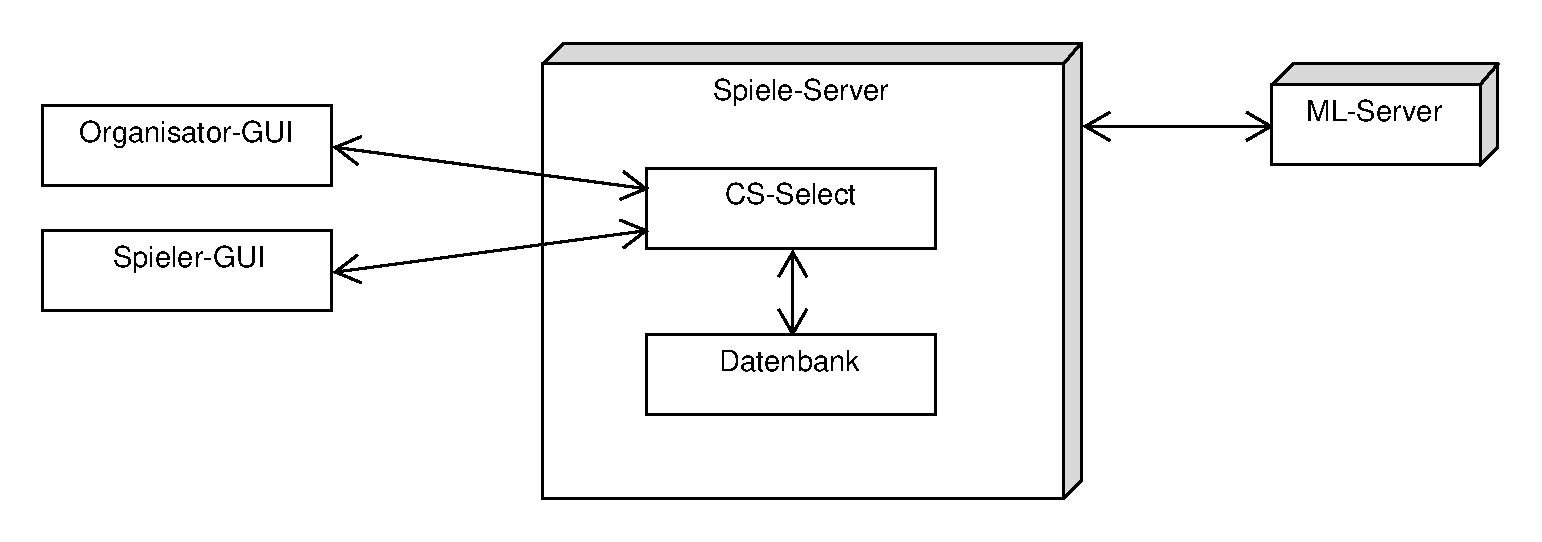
\includegraphics[width=\textwidth]{img/Architektur.pdf}
    Das Produkt wurde nach dem Model-View-Controller-Prinzip entworfen.
	Die Organisator sowie die Spieler-GUI laufen in einem Webbrowser auf dem PC des Nutzers und stellen die View dar.
	Hier interagieren die Spieler und Organisatoren mit dem Produkt.
	Der Spiel-Server koordiniert den Spielablauf, speichert Ergebnisse in der Datenbank ab und kommuniziert mit dem ML-Server.
    In diesem Teil des Produkts finden sich Model und Controller gebündelt.

	\chapter{Änderungen zum Pflichtenheft}
	Im Folgenden werden sämtliche Abweichungen vom Pflichtenheft, die im Entwurf aufgetreten sind, aufgelistet und erläutert.
	\begin{enumerate}
		\item Achievements werden im Gegensatz zu Anforderung /F750/ \emph{nicht} bepunktet. \\Achievements sollen lediglich visuelle Belohnungen darstellen, die sich der Spieler jederzeit anschauen kann.
        \item Das Überspringen einer Runde aus /F500/ hat \emph{keine} Minuspunkte zur Folge, um Demotivation durch Punktabzug eines Spielers zu vermeiden.
		\item Im Zustandsdiagramm Streak aus Abschnitt 9.1.1 des Pflichtenhefts wird eine \\Streak auch beendet, wenn der Spieler eine Runde eines anderen Spiels spielt. Dies ist nicht der Fall. Eine Streak wird auch spielübergreifend erhalten bleiben, denn es geht darum, dass man mehrere Runde am Stück spielt, egal von welchem Spiel. Das aktualisierte Zustandsdiagramm ist in \hyperlink{StreakState}{Abschnitt 7.1} zu finden.
		\item Im Gegensatz zu /F470/ wird vom Organisator bei der Spielerstellung festgelegt, wie viele Merkmale minimal und maximal von einem Spieler ausgewählt werden dürfen.
    \end{enumerate}
	
	\chapter{Klassendiagramme}

	\section{User-Paket}
	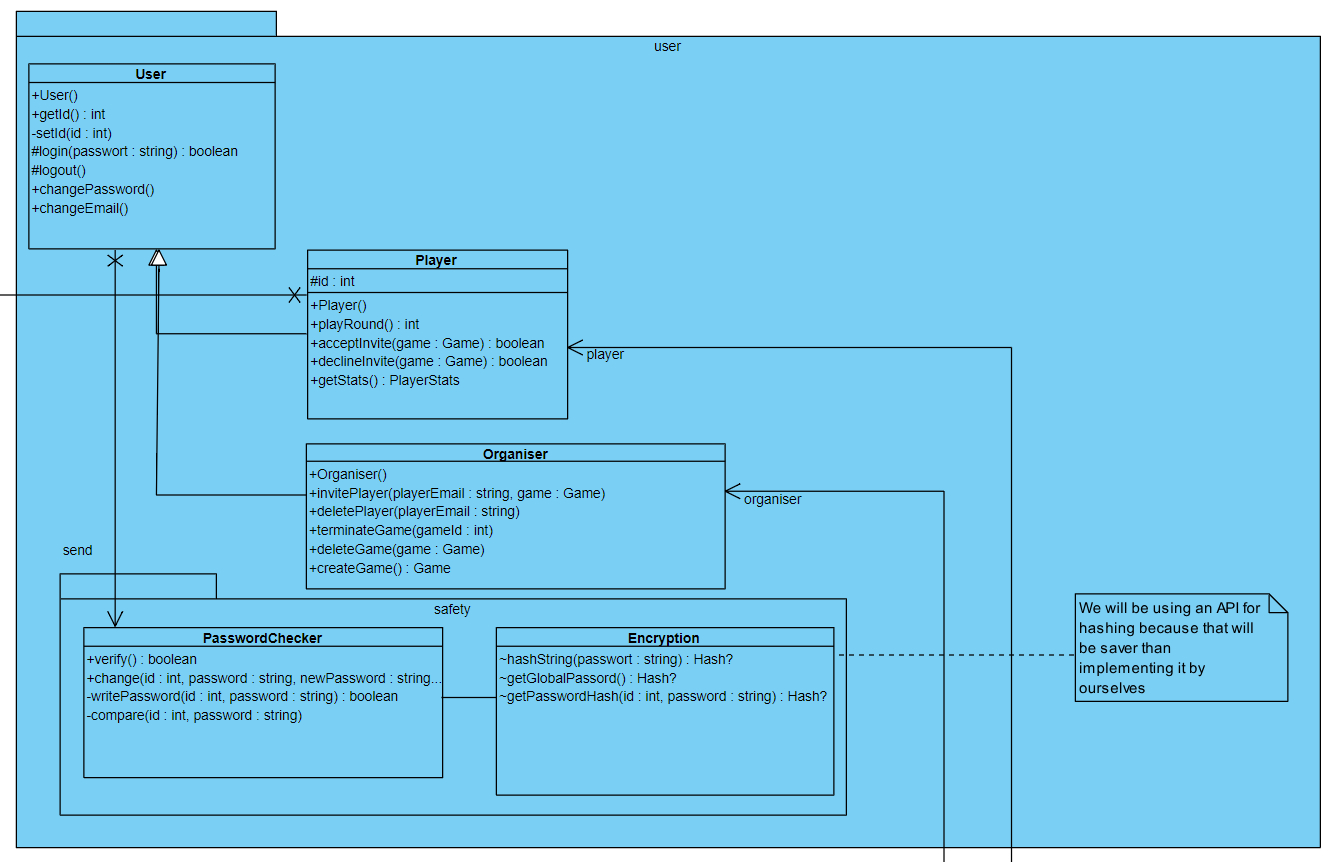
\includegraphics[width=\textwidth]{img/user.png}
	Dieses Paket beinhaltet die Klassen, die im Model-Segment des Programms eine Art Knotenpunkt darstellen. Hat ein Nutzer eine Session, existiert
	eine Fassade, die mit einem Nutzer-Objekt gebunden ist. Nutzer-Objekte werden auch beim Registrieren in der Datenbank erstellt und beim Login
	in das System. Die meisten weiteren Vorgänge im Model werden von Klassen im User-Paket veranlasst (auch durch einfache Weiterleitung der Parameter)
	\subsection{User}
	Stellt einen Nutzer im System dar. Es können mehrere Nutzer-Objekte mit gleicher ID im System zur gleichen Zeit existieren, da der gesamte Datenverkehr über die ständig aktuelle Datenbank verläuft.
		\subsubsection{User}
	\begin{itemize}
		\item Beschreibung: Konstruktor, der einen User mit ID erzeugt
		\item Parameter: int
		\item Rückgabewert: User-Objekt
	\end{itemize}
		\subsubsection{getId}
		\begin{itemize}
			\item Beschreibung: Gibt die eindeutige ID zurück, die einem Nutzer in der Datenbank zugeordnet ist
			\item Rückgabewert: int
		\end{itemize}
		\subsubsection{login}
		\begin{itemize}
			\item Beschreibung: Mithilfe dieser Methode loggt sich der Nutzer ein. Sie gibt einen Boolean zurück, wenn das Passwort mit dem (verschlüsselten) Password in der Datenbank übereinstimmt
			\item Parameter: String
			\item Rückgabewert: boolean
		\end{itemize}
		\subsubsection{logout}
		\begin{itemize}
			\item Beschreibung: Diese Methode dient dem Ausloggen des Nutzers. Der dem Nutzer zugehörige Datenbankadapter wird entkoppelt, Nutzer-Objekt wird später von Garbage-Collector gelöscht
			\item Parameter: -
			\item Rückgabewert: void
		\end{itemize}
		\subsubsection{changePassword}
		\begin{itemize}
			\item Beschreibung: Mit dieser Methode ändert der Nutzer sein Passwort. Über die Kommunikation per Datenbankadapter wird mit der internen Datenbank kommuniziert
			\item Parameter: String
			\item Rückgabewert: void
		\end{itemize}
		\subsubsection{changeEmail}
		\begin{itemize}
			\item Beschreibung: Ermöglicht die Änderung der Email eines Nutzers. Erneut wird die Kommunikation per Datenbankadapter erfolgen
			\item Parameter: String
			\item Rückgabewert: void
		\end{itemize}
	\subsubsection{setLanguage}
	\begin{itemize}
		\item Beschreibung: Ändert die gewünschte Sprache des Spielers, Spachcode wird in der Datenbank vermerkt
		\item Parameter: String
		\item Rückgabewert: void
	\end{itemize}

	\subsection{Player}
	Player stellt den Spieler im System dar. Diese Klasse erbt von der Nutzer-Klasse
		\subsubsection{Player}
		\begin{itemize}
			\item Beschreibung: Konstruktor für Player-Objekte mit (garantiert eindeutiger) Nutzer-ID
			\item Parameter: int
			\item Rückgabewert: Player-Objekt
		\end{itemize}
		\subsubsection{startRound}
		\begin{itemize}
			\item Beschreibung: Methode, um eine neue Runde eines Spiels aufzurufen. Daraufhin wird eine Menge an Merkmalen zurückgeliefert
			\item Parameter: int (Game-ID\footnote{In der Spieler-Klasse werden nur Spiele abgespeichert, denen der Spieler beigetreten ist.} repräsentierend)
			\item Rückgabewert: Collection<Feature>
		\end{itemize}
		\subsubsection{acceptInvite}
		\begin{itemize}
			\item Beschreibung: Ermöglicht Annahme einer Einladung zu einem Spiel mit (eindeutiger) Spiel-ID
			\item Parameter: int
			\item Rückgabewert: void
		\end{itemize}
		\subsubsection{declineInvite}
		\begin{itemize}
			\item Beschreibung: Spieler lehnt Einladung zu einem Spiel mit eindeutiger Spiel-ID ab
			\item Parameter: int
			\item Rückgabewert:
		\end{itemize}
		\subsubsection{getStats}
		\begin{itemize}
			\item Beschreibung: %TODO: Beschreibung
			\item Parameter: -
			\item Rückgabewert: Gamification-Interface
		\end{itemize}
		\subsubsection{selectFeatures}
		\begin{itemize}
			\item Beschreibung: %TODO: Beschreibung
			\item Parameter:
			\begin{itemize}
				\item Collection<Feature>
				\item Collection<Feature>
			\end{itemize}
			\item Rückgabewert: void
		\end{itemize}
		\subsubsection{getLeaderBoard}
		\begin{itemize}
			\item Beschreibung: Gibt eine geordnete Liste an Spielern zurück
			\item Parameter: -
			\item Rückgabewert: List<Player>
		\end{itemize}
		\subsubsection{selectFeatures}
		\begin{itemize}
		\item Beschreibung: Nimmt die vom Nutzer ausgewählten Merkmale und als unnötig markierten Merkmale entgegen und leitet diese an die aktive Runde weiter, gibt die von dieser berechnete Punktzahl zurück an die Fassade.
		\item Parameter:
		\begin{itemize}
		\item selectedFeatures: Die vom Spieler ausgewählten Merkmale
		\item uselessFeatures: Die vom Spieler als unnötig markierten Merkmale
		\end{itemize}
		\end{itemize}

	\subsection{Organiser}
		\subsubsection{Organiser}
		\begin{itemize}
			\item Beschreibung: Konstruktor für Organisator-Objekt mit im System eindeutiger ID
			\item Parameter: int
			\item Rückgabewert: Organiser-Objekt
		\end{itemize}
	\subsubsection{savePattern}
	\begin{itemize}
		\item Beschreibung: Speichert die aktuellen Optionen bei der Spielerstellung
		\item Parameter: String
		\item Rückgabewert: void
	\end{itemize}
	\subsubsection{getPatterns}
	\begin{itemize}
		\item Beschreibung: Liefert alle Patterns zurück, die der Organisator gespeichert hat
		\item Parameter: -
		\item Rückgabewert: Collection<Pattern>
	\end{itemize}
	\subsubsection{loadPattern}
	\begin{itemize}
		\item Beschreibung: Lädt die in der angegebenen Pattern gespeicherten Spielerstellungsoptionen
		\item Parameter: Pattern
		\item Rückgabewert: void
	\end{itemize}
		\subsubsection{createGame}
		\begin{itemize}
			\item Beschreibung: Methode, um ein Spiel zu erstellen
			\item Parameter: -
			\item Rückgabewert: void
		\end{itemize}
	\subsubsection{invitePlayer}
	\begin{itemize}
		\item Beschreibung: Methode, die einen Spieler zu einem Spiel einlädt
		\item Parameter:
		\begin{itemize}
			\item String
			\item String
		\end{itemize}
		\item Rückgabewert: void
	\end{itemize}
		\subsubsection{terminateGame}
		\begin{itemize}
			\item Beschreibung: Aktives Spiel beenden
			\item Parameter: int
			\item Rückgabewert: void
		\end{itemize}
		\subsubsection{deleteGame}
		\begin{itemize}
			\item Beschreibung: Terminiertes Spiel aus der internen Datenbank und somit aus der Übersicht löschen
			\item Parameter: int
			\item Rückgabewert: void
		\end{itemize}

	\section{API}
	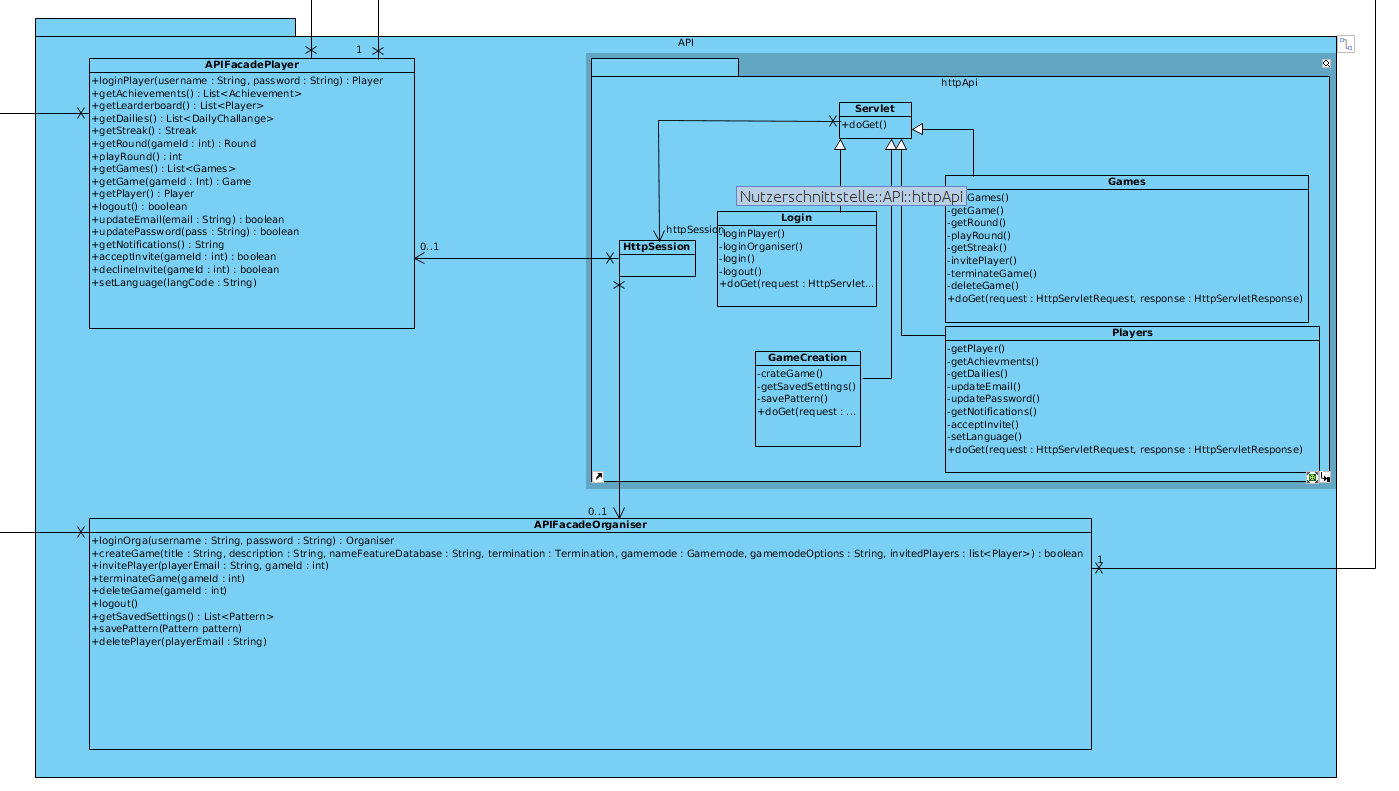
\includegraphics[width=\textwidth]{img/api.png}
	% TODO Hier auch eine Paketbeschreibung \\
	\subsection{APIFacadePlayer}
	Eine APIFacadePlayer ist das Objekt, über welches sämtliche Interaktion mit dem System von den Spielern aus passiert. Nach dem Konstruktor \textbf{muss} zuerst loginPlayer aufgerufen werden, bis es erfolgreich zurückkehrt. Ansonsten haben alle anderen Methoden kein definiertes Verhalten und werden im Allgemeinem nichts Nützliches zurückgeben. Eine APIFacadePlayer ist immer mit einem Spieler assoziiert, falls dieser korrekt angemeldet wurde. Alle Methoden beziehen sich dann auf den angemeldeten Spieler.
	\subsubsection{loginPlayer}
	\begin{itemize}
		\item Beschreibung: Versucht einen Spieler mit email und password anzumelden. Bei Erfolg wird diese Fassade mit dem Spieler assoziiert.
		\item Parameters:
		\begin{itemize}
			\item email: Die E-Mail Adresse, mit der eine Anmeldung versucht wird
			\item password: Das Passwort, mit dem eine Anmeldung versucht wird
		\end{itemize}
		\item Rückgabewert: Falls die E-Mail-Passwort-Kombination einen validen Spieler beschreibt, wird dieser zurückgegeben. Andernfalls wird null zurückgegeben.
	\end{itemize}
	\subsubsection{logout}
	\begin{itemize}
		\item Beschreibung: Meldet den angemeldeten Spieler ab. Nach dem Aufruf dieser Methode verhält sich dieses Objekt wieder so, als ob nie ein Spieler angemeldet wurde
	\end{itemize}
	\subsubsection{getAchievements}
	\begin{itemize}
		\item Beschreibung: Holt die Liste aller Achievements, mit der Information, ob der Spieler diese bereits erreicht hat oder nicht.
		\item Rückgabewert: Liste an Achievements.
	\end{itemize}
	\subsubsection{getLeaderboard}
	\begin{itemize}
		\item Beschreibung: Gibt das aktuelle Leaderboard in der geordneten Reihenfolge zurück
		\item Rückgabewert: Eine Liste an Spielern, geordnet nach ihrer Leaderboard-Ordunung.
	\end{itemize}
	\subsubsection{getDaily}
	\begin{itemize}
		\item Beschreibung: Gibt die Daily-Challenge für diesen Spieler zurück.
		\item Rückgabewert: Die aktuelle Daily-Challenge.
	\end{itemize}
	\subsubsection{getStreak}
	\begin{itemize}
		\item Beschreibung: Gibt das aktuelle Streak-Objekt für diesen Spieler zurück
		\item Rückgabewert: Das aktuelle Streak-Objekt für diesen Spieler
	\end{itemize}
	\subsubsection{getPoints}
	\begin{itemize}
		\item Beschreibung: Gibt die Punkte des Spielers zurück
		\item Rückgabewert: Aktuelle Punktzahl des Spielers
	\end{itemize}
	\subsubsection{getRound}
	\begin{itemize}
		\item Beschreibung: Fordert die nächste Runde für ein Spiel an und gibt diese zurück
		\item Parameter:
		\begin{itemize}
			\item gameId: Eindeutige Id des Spieles für das die Runde angefordert wird
		\end{itemize}
		\item Rückgabewert: Wenn der Spieler eine Runde in dem angegebenem Spiel spielen darf, dann wird das Runden-Objekt zurückgegen. Andernfalls wird null zurückgegeben
	\end{itemize}
	\subsubsection{playRound}
	\begin{itemize}
		\item Beschreibung: Spielt eine Runde in der aktuellen Runde
	\end{itemize}
	\subsubsection{getGames}
	\begin{itemize}
		\item Beschreibung: Holt alle Spiele, an denen der Spieler teilnimmt
		\item Rückgabewert: Liste an Spielen, an denen der Spieler teilnimmt
	\end{itemize}
	\subsubsection{getGame}
	\begin{itemize}
		\item Beschreibung: Gibt ein Spiel nach Id zurück, falls der Spieler auf dieses Spiel Zugriff hat
		\item Parameter:
		\begin{itemize}
			\item gameId: die Id des Spiels, welches zurückgegeben werden soll
		\end{itemize}
		\item Rückgabewert: Falls gameId valid ist, also Spiel existiert und Spieler darf auf das Spiel zugreifen, dann wird das Spiel zurückgegen, ansonsten null.
	\end{itemize}
	\subsubsection{getPlayer}
	\begin{itemize}
		\item Beschreibung: Gibt den angemeldeten Spieler zurück. Also der Spieler, welcher durch loginPlayer angemeldet wurde.
		\item Rückgabewert: Der angemeldete Spieler, falls keiner angemeldet ist wird null zurückgegeben.
	\end{itemize}
	\subsubsection{changeEmail}
	\begin{itemize}
		\item Beschreibung: Ändert die E-Mail-Adresse mit der sich ein Spieler anmeldet. Die Änderung tritt erst in Effekt, wenn die neue E-Mail-Adresse bestätigt wurde.
		\item Parameter:
		\begin{itemize}
			\item email: Die neue E-Mail-Adresse, welche in Zukunft für diesen Spieler verwendet werden soll.
		\end{itemize}
		\item Rückgabewert: true, falls die Bestätigungsmail veschickt wurde, false andernfalls
	\end{itemize}
	\subsubsection{changePassword}
	\begin{itemize}
		\item Beschreibung: Ändert das Passwort, mit dem sich der Spieler anmeldet. Die Änderung tritt sofort in Effekt.
		\item Parameter:
		\begin{itemize}
			\item pass: Das neue Passwort
		\end{itemize}
		\item Rückgabewert: true falls die Änderung erfolgreich war, false andernfalls
	\end{itemize}
	\subsubsection{getNotifications}
	\begin{itemize}
		\item Beschreibung: Holt alle Notifications, die für diesen Spieler anliegen
		\item Rückgabewert:  Alle Notifications, die für diesen Spieler anliegen
	\end{itemize}
	\subsubsection{acceptInvite}
	\begin{itemize}
		\item Beschreibung: Akzeptiert eine Einladung zu einem Spiel, welche diesem Spieler geschickt wurde und löscht diese aus seinen Einladungen
		\item Parameter:
		\begin{itemize}
			\item gameId: Id des Spiels für das die Einladung angenommen werden soll.
		\end{itemize}
		\item Rückgabewert: true wenn die Einladung angenommen wurde, false falls der Spieler keine Einladung zu diesem Spiel hatte, das Spiel nicht existier oder bereits beendet ist.
	\end{itemize}
	\subsubsection{declineInvite}
	\begin{itemize}
		\item Beschreibung: Lehnt eine Einladung zu einem Spiel ab, welche diesem Spieler geschickt wurde und löscht diese aus seinen Einladungen
		\item Parameter:
		\begin{itemize}
			\item gameId: Id des Spiels für das die Einladung abgelehnt werden soll.
		\end{itemize}
		\item Rückgabewert: true, wenn die Einladung abgelehnt wurde, false, falls der Spieler keine Einladung zu diesem Spiel hatte, das Spiel nicht existiert oder bereits beendet ist.
	\end{itemize}
	\subsubsection{setLanguage}
	\begin{itemize}
		\item Beschreibung: Setzt die Sprache für den Spieler
		\item Parameter:
		\begin{itemize}
			\item langCode: der Landescode für die gewünschte Sprache
		\end{itemize}
	\end{itemize}
    \subsubsection{registerPlayer}
    \begin{itemize}
        \item Beschreibung: registriert einen neuen Spieler in das System. Bei diesem Aufruf wird eine E-Mail an die angegebene Email gesendet. Das Passwort muss der Spieler sich merken, da es in den loginPlayer Aufruf benötigt wird.
        \item Parameter:
        \begin{itemize}
            \item email: E-Mail Adresse des zu registrierenden Spielers. Der Spieler muss Zugriff auf diese E-Mail Adresse haben.
            \item password: Das Passwort des neu zu registrierenden Spielers.
            \item username: Der Nutzername des neu zu registrierenden Spielers.
        \end{itemize}
    \end{itemize}
    \subsubsection{validateEmail}
    \begin{itemize}
        \item Beschreibung: Teilt dem System mit, dass die E-Mail Adresse eines Nutzers bestätigt wurde. Optimalerweise durch den Link, welcher in der E-Mail versendet wurde. Kann aber natürlich auf direkt nach dem registerPlayer Aufruf gemacht werden.
    \end{itemize}
	\subsection{APIFacadeOrganiser}
	\subsubsection{loginOrganiser}
	\begin{itemize}
		\item Beschreibung: meldet einen Organisator an. Damit dies möglich ist, muss der Organisator vorher registriert worden sein.
		\item Parameter:
		\begin{itemize}
			\item email: E-Mail des anzumeldenden Organisators
			\item password: Das Passwort des anzumeldenden Organisators
		\end{itemize}
		\item Rückgabewert: Falls die Email-Passwort Kombinnation valid ist, also ein Organisator mit der E-Mail registriert ist und das Passwort ist richtig, wird der Organisator zurückgegeben. Andernfalls null.
	\end{itemize}
	\subsubsection{createGame}
	\begin{itemize}
		\item Beschreibung: erstellt ein Spiel für diesen Organisator.
		\item Parameter: %% stuff bleibt hier ja noch nicht ganz fest gegeben
		\begin{itemize}
			\item :
		\end{itemize}
		\item Rückgabewert: Falls das Erstellen erfolgreich war, true zurückgegeben, andernfalls false.
	\end{itemize}
	\subsubsection{invitePlayer}
	\begin{itemize}
		\item Beschreibung: Lädt einen Spieler zu einem Spiel des Organisators ein.
		\item Parameter:
		\begin{itemize}
			\item playerEmail: die Email-Adresse des einzuladenden Spielers
			\item gameId: Das Spiel, zu dem der Spieler eingeladen werden soll. Das Spiel muss ein Spiel des Organisators sein.
		\end{itemize}
	\end{itemize}
	\subsubsection{terminateGame}
	\begin{itemize}
		\item Beschreibung: Beendet ein Spiel des Organisators.
		\item Parameter:
		\begin{itemize}
			\item gameId: Id des zu beendenden Spiels. Das Spiel muss zu dem Organisator gehören.
		\end{itemize}
	\end{itemize}
	\subsubsection{deleteGame}
	\begin{itemize}
		\item Beschreibung: Löscht ein Spiel des Organisators aus dem System.
		\item Parameter:
		\begin{itemize}
			\item gameId: Die Id des zu löschenden Spiel
		\end{itemize}
	\end{itemize}
	\subsubsection{logout}
	\begin{itemize}
		\item Beschreibung: Meldet einen Organisator ab. Nach dem Aufruf dieser Methode verhält sich dieses Objekt so, als ob niemand angemeldet war.
	\end{itemize}
	\subsubsection{getSavedSettings}
	\begin{itemize}
		\item Beschreibung: Holt eine Liste aller gespeicherten Einstellungen dieses Organisators.
		\item Rückgabewert: Eine Liste aller gespeichterten Einstellungen dieses Organisators.
	\end{itemize}
	\subsubsection{savePattern}
	\begin{itemize}
		\item Beschreibung: Speichert eine Einstellungskonfiguration für diesen Organisator
		\item Parameter:
		\begin{itemize}
			\item pattern: Das zu speichernde Pattern
		\end{itemize}
	\end{itemize}
	\subsubsection{registerOrganiser}
    \begin{itemize}
        \item Beschreibung: registriert einen neuen Spieler in das System. Bei diesem Aufruf wird eine E-Mail an die angegebene Email gesendet. Das Passwort muss der Spieler sich merken, da es in den loginOrganiser Aufruf benötigt wird.
        \item Parameter:
        \begin{itemize}
            \item email: E-Mail Adresse des zu registrierenden Organisators. Der Organisator muss Zugriff auf diese E-Mail Adresse haben.
            \item password: Das Passwort des neu zu registrierenden Organisators.
            \item mainPassword: Das Haupt-Passwort, welches in der Konfigurationsdatei steht und benötigt wird um das registrieren als Organisator zu erlauben.
        \end{itemize}
    \end{itemize}
    \subsubsection{validateEmail}
    \begin{itemize}
        \item Beschreibung: Teilt dem System mit, dass die E-Mail Adresse eines Nutzers bestätigt wurde. Optimalerweise durch den Link, welcher in der E-Mail versendet wurde. Kann aber natürlich auf direkt nach dem registerOrganiser Aufruf gemacht werden.
    \end{itemize}
    \subsection{httpAPI}
    Implementierung der beiden Fassadenobjecten für http/REST.

	\section{Database}
	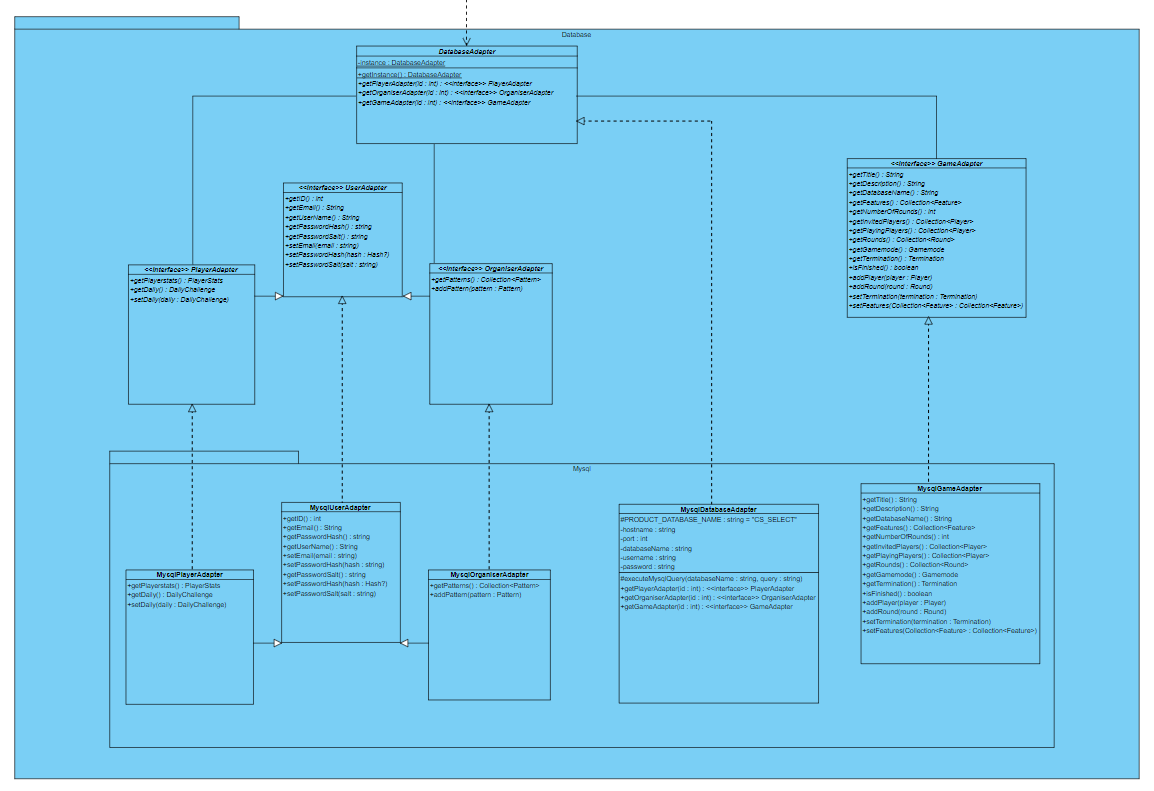
\includegraphics[width=\textwidth]{img/Database.PNG}
	Paket, das die Kommunikation mit der Datenbank übernimmt.

	\subsection{DatabaseAdapter}
	Abstrakte Klasse, die als Singleton realisiert ist und von der jeweiligen Datenbankimplementierung abstrahiert.
	In der getInstance Methode wird anhand des in der Konfiguration angegebenen Datenbanktyps die Implementierung ausgewählt.

	\subsubsection{instance}
	Instanz des Singletons, die durch Vererbung spezialisiert wird.

	\subsubsection{getInstance}
	\begin{itemize}
		\item Beschreibung: Statische Methode, die die Instanz des DatabaseAdapters zurückgibt.
		\item Rückgabewert: Instanz des DatabaseAdapters.
	\end{itemize}

	\subsubsection{getPlayerAdapter}
	\begin{itemize}
		\item Beschreibung: Gibt den PlayerAdapter für den Spieler mit der gegebenen ID zurück.
		\item Parameter:
		\begin{itemize}
			\item id: ID des Spielers, dessen PlayerAdapter zurückgegeben werden soll.
		\end{itemize}
		\item Rückgabewert: PlayerAdapter des Spielers mit ID id.
	\end{itemize}

	\subsubsection{getOrganiserAdapter}
	\begin{itemize}
		\item Beschreibung: Gibt den OrganiserAdapter für den Organisator mit der gegebenen ID zurück.
		\item Parameter:
		\begin{itemize}
			\item id: ID des Organisators, dessen OrganiserAdapter zurückgegeben werden soll.
		\end{itemize}
		\item Rückgabewert: OrganiserAdapter des Organisators mit ID id.
	\end{itemize}

	\subsubsection{getGameAdapter}
	\begin{itemize}
		\item Beschreibung: Gibt den GameAdapter für das Spiel mit der gegebenen ID zurück.
		\item Parameter:
		\begin{itemize}
			\item id: ID des Spiels, dessen GameAdapter zurückgegeben werden soll.
		\end{itemize}
		\item Rückgabewert: GameAdapter des Spiels mit ID id.
	\end{itemize}

	\subsubsection{getPlayer}
	\begin{itemize}
		\item Beschreibung: Gibt das Player Objekt mit der gegebenen E-Mail-Addresse zurück.
		\item Parameter:
		\begin{itemize}
			\item email: E-Mail-Addresse des Spielers der zurückgegeben werden soll.
		\end{itemize}
		\item Rückgabewert: Player mit der gegebenen E-Mail-Addresse
	\end{itemize}


	\subsubsection{getOrganiser}
	\begin{itemize}
		\item Beschreibung: Gibt das Organiser Objekt mit der gegebenen E-Mail-Addresse zurück.
		\item Parameter:
		\begin{itemize}
			\item email: E-Mail-Addresse des Organisers der zurückgegeben werden soll.
		\end{itemize}
		\item Rückgabewert: Organiser mit der gegebenen E-Mail-Addresse
	\end{itemize}

	\subsubsection{getPlayers}
	\begin{itemize}
		\item Beschreibung: Gibt alle gespeicherten Spieler zurück.
		\item Rückgabewert: Collection aller gespeicherten Spieler.
	\end{itemize}

    \subsubsection{getNextGameID}
    \begin{itemize}
        \item Beschreibung: Gibt die ID zurück die das nächste zu speichernde Spiel erhalten muss.
        \item Rückgabewert: ID des nächsten zu speichernden Spiels.
    \end{itemize}

	\subsubsection{getActiveGames}
	\begin{itemize}
		\item Beschreibung: Gibt die aktiven Spiele des gegebenen Organisators zurück.
		\item Parameter:
		\begin{itemize}
			\item organiser: Organisator dessen Spiele zurückgegeben werden sollen.
		\end{itemize}
		\item Rückgabewert: Collection der aktiven Spiele.
	\end{itemize}

	\subsubsection{getTerminatedGames}
	\begin{itemize}
		\item Beschreibung: Gibt die terminierten Spiele des gegebenen Organisators zurück.
		\item Parameter:
		\begin{itemize}
			\item organiser: Organisator dessen Spiele zurückgegeben werden sollen.
		\end{itemize}
		\item Rückgabewert: Collection der terminierten Spiele.
	\end{itemize}

	\subsubsection{registerPlayer}
	\begin{itemize}
		\item Beschreibung: Fügt einen neuen Spieler zur Datenbank hinzu und gibt ihn zurück.
		\item Parameter:
		\begin{itemize}
			\item username: Nutzername des zu speichernden Spielers.
			\item email: E-Mail-Addresse des zu speichernden Spielers.
			\item password: Passwort des zu speichernden Spielers.
		\end{itemize}
		\item Rückgabewert: Angelegter Spieler.
	\end{itemize}

	\subsubsection{registerOrganiser}
	\begin{itemize}
		\item Beschreibung: Fügt einen neuen Organisator zur Datenbank hinzu und gibt ihn zurück.
		\item Parameter:
		\begin{itemize}
			\item username: Nutzername des zu speichernden Spielers
			\item email: E-Mail-Addresse des zu speichernden Organisators.
			\item password: Passwort des zu speichernden Organisators.
			\item givenOrganiserPassword: Vom Organisator eingegebenes Organisator-Passwort, wird auf Korrektheit überprüft.
		\end{itemize}
		\item Rückgabewert: Angelegter Organisator.
	\end{itemize}

	\subsubsection{registerGame}
	\begin{itemize}
		\item Beschreibung: Fügt ein neues Spiel das dem gegebenen Organisator gehört zur Datenbank hinzu.
		\item Parameter:
		\begin{itemize}
			\item organiser: Organisator dem das Spiel gehört.
			\item game: Spiel das gespeichert werden soll.
		\end{itemize}
	\end{itemize}

	\subsubsection{removeGame}
	\begin{itemize}
		\item Beschreibung: Entfernt das gegebene Spiel aus der Hauptdatenbank des Produkts.
		Die Ergebnisse in der spieleigenen Datenbank bleiben unangetastet.
		\item Parameter:
		\begin{itemize}
			\item game: Spiel das aus der Datenbank entfernt werden soll.
		\end{itemize}
	\end{itemize}

	\subsection{UserAdapter}
	Schnittstelle die Methoden für alle Nutzer des Produkts bereitstellt.
	Jeder UserAdapter ist genau einem Nutzer zugeordnet.

	\subsubsection{getID}
	\begin{itemize}
		\item Beschreibung: Gibt die ID des Nutzers zurück.
		\item Rückgabewert: int mit ID des Nutzers.
	\end{itemize}

	\subsubsection{getEmail}
	\begin{itemize}
		\item Beschreibung: Gibt die E-Mail-Addresse des Nutzers zurück.
		\item Rückgabewert: String mit E-Mail-Addresse des Nutzers.
	\end{itemize}

	\subsubsection{getPasswordHash}
	\begin{itemize}
		\item Beschreibung: Gibt das gehashte Passwort des Nutzers zurück.
		\item Rückgabewert: Hash des Passworts
	\end{itemize}

	\subsubsection{setEmail}
	\begin{itemize}
		\item Beschreibung: Setzt die E-Mail-Adresse des Nutzers neu.
		\item Parameter:
		\begin{itemize}
			\item email: String der neuen E-Mail-Adresse.
		\end{itemize}
	\end{itemize}

	\subsubsection{setPassword}
	\begin{itemize}
		\item Beschreibung: Setzt das gehashte Passwort sowie den Salt des Nutzers neu.
		\item Parameter:
		\begin{itemize}
			\item hash: Hash-String des neuen Passworts
			\item salt: Salt-String des neuen Passworts
		\end{itemize}
	\end{itemize}

	\subsubsection{getLanguage}
	\begin{itemize}
		\item Beschreibung: Gibt die Sprache des Nutzers zurück.
		\item Rückgabewert: String der Sprache.
	\end{itemize}

	\subsubsection{setLanguage}
	\begin{itemize}
		\item Beschreibung: Setzt die Sprache des Nutzers neu.
		\item Parameter:
		\begin{itemize}
			\item email: String der neuen Sprache.
		\end{itemize}
	\end{itemize}

	\subsection{PlayerAdapter}
	Schnittstelle die UserAdapter erweitert.
	Jeder PlayerAdapter ist stets genau einem Spieler zugeordnet.

    \subsubsection{getUsername}
    \begin{itemize}
        \item Beschreibung: Gibt den Nutzernamen des Nutzers zurück.
        \item Rückgabewert: String mit Nutzernamen des Nutzers.
    \end{itemize}

	\subsubsection{getPlayerStats}
	\begin{itemize}
		\item Beschreibung: Gibt die gespeicherten PlayerStats eines Spielers zurück.
		\item Rückgabewert: PlayerStats Objekt des Spielers.
	\end{itemize}

	\subsubsection{getDaily}
	\begin{itemize}
		\item Beschreibung: Gibt die aktuelle Daily Challenge des Spielers zurück.
		\item Rückgabewert: Aktuelles DailyChallenge Objekt.
	\end{itemize}

	\subsubsection{setDaily}
	\begin{itemize}
		\item Beschreibung: Setzt die Daily-Challenge des Spielers neu.
		\item Parameter:
		\begin{itemize}
			\item daily: Zu setzende Daily-Challenge
		\end{itemize}
	\end{itemize}
	\subsubsection{getGames}
	\begin{itemize}
		\item Beschreibung: Gibt alle Spiele zu denen der Spieler zugeordnet ist zurück.
		\item Rückgabewert: Collection aller Spiele denen ein Spieler zugeordnet ist.
	\end{itemize}

	\subsection{OrganiserAdapter}
	Schnittstelle die UserAdapter erweitert.
	Jeder OrganiserAdapter ist stets genau einem Organisator zugeordnet.

	\subsubsection{getPatterns}
	\begin{itemize}
		\item Beschreibung: Gibt die gespeicherten Patterns des Organisators zurück.
		\item Rückgabewert: Collection der gespeicherten Patterns des Organisators.
	\end{itemize}

	\subsubsection{addPatterns}
	\begin{itemize}
		\item Beschreibung: Speichert eine Spielvoreinstellung für den Organisator ab.
		\item Parameter:
		\begin{itemize}
			\item pattern: Zu speichernde Spielvoreinstellung.
		\end{itemize}
	\end{itemize}

	\subsubsection{getActiveGames}
	\begin{itemize}
		\item Beschreibung: Gibt die aktiven Spiele des gegebenen Organisators zurück.
		\item Parameter:
		\begin{itemize}
			\item organiser: Organisator dessen Spiele zurückgegeben werden sollen.
		\end{itemize}
		\item Rückgabewert: Collection der aktiven Spiele.
	\end{itemize}

	\subsubsection{getTerminatedGames}
	\begin{itemize}
		\item Beschreibung: Gibt die terminierten Spiele des gegebenen Organisators zurück.
		\item Parameter:
		\begin{itemize}
			\item organiser: Organisator dessen Spiele zurückgegeben werden sollen.
		\end{itemize}
		\item Rückgabewert: Collection der terminierten Spiele.
	\end{itemize}

	\subsection{GameAdapter}
	Schnittstelle die Methoden für gespeicherte Spiele des Produkts bereitstellt.
	Jeder GameAdapter ist stets genau einem Spiel zugeordnet.

	\subsubsection{getTitle}
	\begin{itemize}
		\item Beschreibung: Gibt den Titel des Spiels zurück.
		\item Rückgabewert: String mit Titel.
	\end{itemize}

	\subsubsection{getDescription}
	\begin{itemize}
		\item Beschreibung: Gibt die Beschreibung des Spiels zurück.
		\item Rückgabewert: String mit Beschreibung des Spiels.
	\end{itemize}

	\subsubsection{getDatabaseName}
	\begin{itemize}
		\item Beschreibung: Gibt den Namen der Datenbank zurück in der das Spiel gespeichert ist.
		\item Rückgabewert: String mit Namen der Datenbank.
	\end{itemize}

	\subsubsection{getFeatures}
	\begin{itemize}
		\item Beschreibung: Gibt die Features des Spiels zurück.
		\item Rückgabewert: FeatureSet mit den Features des Spiels
	\end{itemize}

	\subsubsection{getNumberOfRounds}
	\begin{itemize}
		\item Beschreibung: Gibt die Anzahl der zu spielenden Runden zurück.
		\item Rückgabewert: int mit zu spielenden Runden.
	\end{itemize}

	\subsubsection{getInvitedPlayers}
	\begin{itemize}
		\item Beschreibung: Gibt die eingeladenen Spieler zurück.
		\item Rückgabewert: Collection mit den eingeladenen Spielern
	\end{itemize}

	\subsubsection{getPlayingPlayers}
	\begin{itemize}
		\item Beschreibung: Gibt die spielenden Spieler zurück.
		\item Rückgabewert: Collection mit den spielenden Spielern.
	\end{itemize}

	\subsubsection{getRounds}
	\begin{itemize}
		\item Beschreibung: Gibt die gespielten Runden zurück.
		\item Rückgabewert: Collection der gespielten Runden.
	\end{itemize}

	\subsubsection{getGamemode}
	\begin{itemize}
		\item Beschreibung: Gibt den gewählten Spielmodus zurück.
		\item Rückgabewert: Gamemode
	\end{itemize}

	\subsubsection{getTermination}
	\begin{itemize}
		\item Beschreibung: Gibt die Art der Spielterminierung zurück.
		\item Rückgabewert: Termination
	\end{itemize}

	\subsubsection{getOrganiser}
	\begin{itemize}
		\item Beschreibung: Gibt den Organisator zurück dem das Spiel gehört.
		\item Rückgabewert: Organiser
	\end{itemize}

	\subsubsection{isFinished}
	\begin{itemize}
		\item Beschreibung: Gibt zurück ob das Spiel beendet wurde oder nicht.
		\item Rückgabewert: True falls das Spiel beendet wurde, false sonst
	\end{itemize}

	\subsubsection{addPlayer}
	\begin{itemize}
		\item Beschreibung: Fügt einen Spieler zum Spiel hinzu.
		\item Parameter:
		\begin{itemize}
			\item email: E-Mail des Spielers der hinzugefügt werden soll.
			Hier ist die E-Mail statt einem Player Objekt erforderlich da Spieler auch zu Spielen eingeladen werden können wenn sie noch nicht im System registriert sind.
		\end{itemize}
	\end{itemize}

	\subsubsection{addRound}
	\begin{itemize}
		\item Beschreibung: Fügt eine Runde zum Spiel hinzu.
		\item Parameter:
		\begin{itemize}
			\item round: Runde die hinzugefügt werden soll.
		\end{itemize}
	\end{itemize}

	\subsubsection{setTermination}
	\begin{itemize}
		\item Beschreibung: Setzt die Art der Spielterminierung.
		\item Parameter:
		\begin{itemize}
			\item termination: Termination Objekt das die Art der Spielterminierung festlegt.
		\end{itemize}
	\end{itemize}

	\subsubsection{setFeatures}
	\begin{itemize}
		\item Beschreibung: Setzt die Features des Spiels.
		\item Parameter:
		\begin{itemize}
			\item featureSet: Zu setzendes FeatureSet
		\end{itemize}
	\end{itemize}

	\subsubsection{setFinished}
	\begin{itemize}
		\item Beschreibung: Setzt das Spiel auf beendet.
	\end{itemize}

	\subsubsection{setTitle}
	\begin{itemize}
        \item Beschreibung: Setzt den Titel des Spiels.
        \item Parameter:
        \begin{itemize}
            \item title: Zu setzender Titel des Spiels.
        \end{itemize}
	\end{itemize}

	\subsubsection{setDescription}
    \begin{itemize}
        \item Beschreibung: Setzt den Titel des Spiels.
        \item Parameter:
        \begin{itemize}
            \item title: Zu setzender Titel des Spiels.
        \end{itemize}
    \end{itemize}

    \subsubsection{setDatabase}
    \begin{itemize}
        \item Beschreibung: Setzt die Beschreibung des Spiels.
        \item Parameter:
        \begin{itemize}
            \item title: Zu setzende Beschreibung des Spiels.
        \end{itemize}
    \end{itemize}

	\subsubsection{setGamemode}
    \begin{itemize}
        \item Beschreibung: Setzt den Spielmodus des Spiels.
        \item Parameter:
        \begin{itemize}
            \item title: Zu setzender Spielmodus.
        \end{itemize}
    \end{itemize}

	\subsubsection{setOrganiser}
	\begin{itemize}
		\item Beschreibung: Setzt den Organisator dem das Spiel gehört.
		Da Organisatoren nicht nachträglich verändert werden sollen ist die Methode protected, um den Zugriff auf das Datenbank Paket zu beschränken.
		\item Parameter:
		\begin{itemize}
			\item title: Zu setzender Organisator.
		\end{itemize}
	\end{itemize}

	\subsubsection{addInvitedPlayers}
    \begin{itemize}
        \item Beschreibung: Fügt die gegebenen Spieler zu den eingeladenen Spielern hinzu.
        \item Parameter:
        \begin{itemize}
			\item mails: E-Mail-Adressen der Spieler.
        \end{itemize}
    \end{itemize}

	\subsubsection{addPlayingPlayers}
	\begin{itemize}
		\item Beschreibung: Fügt die gegebenen Spieler zu den spielenden Spielern hinzu und entfernt sie gegebenenfalls aus den Eingeladenen.
		\item Parameter:
		\begin{itemize}
			\item mails: E-Mail-Adressen der Spieler.
		\end{itemize}
	\end{itemize}
	
	\subsubsection{removeInvitedPlayers}
	\begin{itemize}
	\item Beschreibung: Entfernt die angegebenen Spieler aus den eingeladenen Spielern
			\item Parameter:
			\begin{itemize}
				\item mails: E-Mail-Adressen der Spieler.
			\end{itemize}
	\end{itemize}

	\subsection{Mysql}
	Paket mit Mysql basierter Implementierung der Datenbank.
	Mitgelieferte Standard-Implementierung des Produkts.

	\subsubsection{MysqlDatabaseAdapter}
	Mysql Implementierung der DatabaseAdapter Klasse.

	\paragraph{PRODUCT\_DATABASE\_NAME}
	Konstante die den Namen der Hauptdatenbank des Produkts enthält.
	Standardmäßig ist dieser Name CS\_SELECT.

	\paragraph{executeMysqlQuery}
	\begin{itemize}
		\item Beschreibung: Führt den gegebenen Mysql Query auf der Hauptdatenbank des Produkts aus.
		\item Parameter:
		\begin{itemize}
			\item query: Auszuführender Mysql-Query
		\end{itemize}
		\item Rückgabewert: ResultSet mit den geladenen Daten, soll nichts zurückgegeben werden Null.
	\end{itemize}

	\paragraph{executeMysqlQuery}
	\begin{itemize}
		\item Beschreibung: Führt den gegebenen Mysql Query auf der Datenbank mit dem gegebenen Namen aus.
		\item Parameter:
		\begin{itemize}
			\item databaseName: Name der zu nutzenden Datenbank
			\item query: Auszuführender Mysql-Query
		\end{itemize}
        \item Rückgabewert: ResultSet mit den geladenen Daten, soll nichts zurückgegeben werden Null.
	\end{itemize}

	\subsubsection{MysqlUserAdapter}
	Mysql Implementierung der UserAdapter Schnittstelle.

	\subsubsection{MysqlPlayerAdapter}
	Mysql Implementierung der PlayerAdapter Schnittstelle.
	Erbt von MysqlUserAdapter

	\subsubsection{MysqlOrganiserAdapter}
	Mysql Implementierung der OrganiserAdapter Schnittstelle.
	Erbt von MysqlUserAdapter

	\subsubsection{MysqlGameAdapter}
	Mysql Implementierung der GameAdapter Schnittstelle.

	\section{Configuration}
	Paket für die Kommunikation mit der Konfigurationsdatei.

	\subsection{Configuration}
	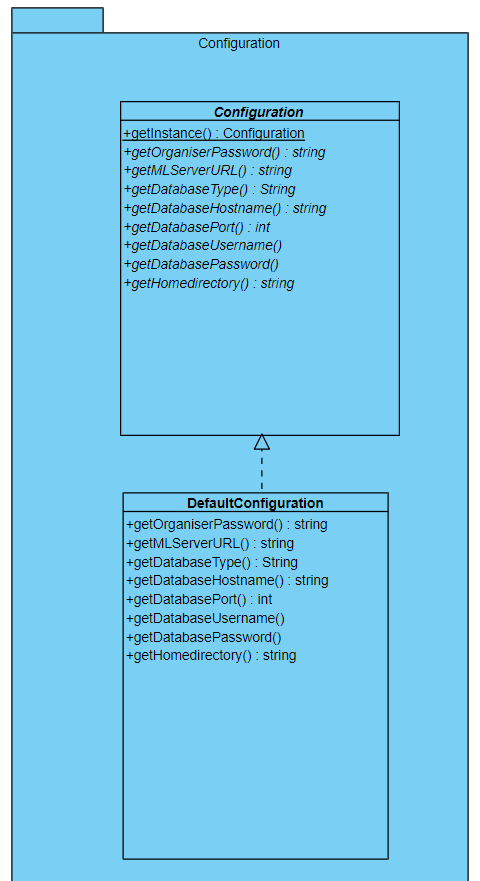
\includegraphics[width=\textwidth]{img/Configuration.PNG}
	Abstrakte Klasse, die von der Config-Implementierung abstrahiert.
	Kümmert sich um die Kommunikation des Produkts mit der Konfigurationsdatei. \\
	Ist als Singleton umgesetzt, um zu erzwingen, dass stets nur ein Zugriffspunkt zur Konfiguration besteht.

	\subsubsection{getInstance}
	\begin{itemize}
		\item Beschreibung: Statische Methode die die Instanz der Configuration zurückgibt.
		\item Rückgabewert: Instanz der Configuration.
	\end{itemize}


	\subsubsection{getOrganiserPassword}
	\begin{itemize}
		\item Beschreibung: Gibt das Passwort als String zurück das Organisatoren bei der Erstregistrierung verwenden müssen.
		\item Rückgabewert: String mit Organisatorpasswort
	\end{itemize}

	\subsubsection{getMLServerURL}
	\begin{itemize}
		\item Beschreibung: Gibt die URL als String zurück, unter der der ML-Server zu finden ist
		\item Rückgabewert: String mit URL des ML-Servers
	\end{itemize}

	\subsubsection{getDatabaseType}
	\begin{itemize}
		\item Beschreibung: Gibt die Art der verwendeten Datenbankimplementierung zurück.
		\item Rückgabewert: String mit Name der Datenbankimplementierung.
	\end{itemize}

	\subsubsection{getDatabaseHostname}
	\begin{itemize}
		\item Beschreibung: Gibt den Hostnamen des Datenbankservers zurück.
		\item Rückgabewert: String mit Hostnamen des Datenbankservers.
	\end{itemize}

	\subsubsection{getDatabasePort}
	\begin{itemize}
		\item Beschreibung: Gibt den Port des Datenbankservers zurück.
		\item Rückgabewert: int mit Port des Datenbankservers.
	\end{itemize}

	\subsubsection{getDatabaseUsername}
	\begin{itemize}
		\item Beschreibung: Gibt den Nutzernamen mit dem sich am Datenbankserver angemeldet wird zurück.
		\item Rückgabewert: String mit Nutzernamen
	\end{itemize}

	\subsubsection{getDatabasePassword}
	\begin{itemize}
		\item Beschreibung: Gibt das Passwort mit dem sich am Datenbankserver angemeldet wird zurück.
		\item Rückgabewert: String mit Passwort
	\end{itemize}

	\subsection{DefaultConfiguration}
	Implementiert die abstrakte Klasse Configuration und stellt die Funktionalität bereit.
	Mitgelieferte Standardimplementierung der Konfiguration.

	\section{MLServer}
	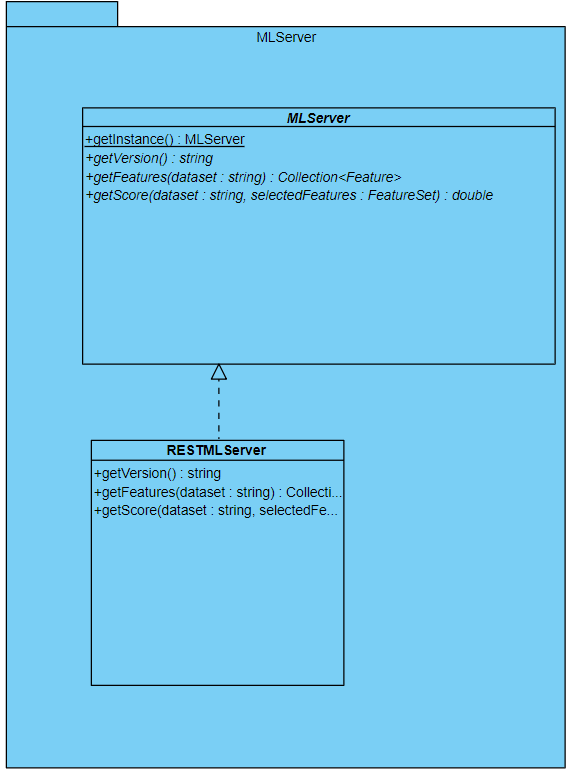
\includegraphics[width=\textwidth]{img/MLServer.PNG}
	Paket für die Kommunikation mit dem ML-Server.

	\subsection{MLServer}
	Abstrakte Klasse die von der Implementierung der ML-Server-API abstrahiert.
	Ist als Singleton umgesetzt um zu erzwingen dass stets nur ein Zugriffspunkt zum ML-Server existiert.

	\subsubsection{getInstance}
	\begin{itemize}
		\item Beschreibung: Statische Methode die die Instanz des MLServers zurückgibt.
		\item Rückgabewert: Instanz des MLServers.
	\end{itemize}

	\subsubsection{getVersion}
	\begin{itemize}
		\item Beschreibung: Gibt die Version des genutzten ML-Servers als String zurück.
		\item Rückgabewert: String mit der Versionsnummer.
	\end{itemize}

	\subsubsection{getFeatures}
	\begin{itemize}
		\item Beschreibung: Gibt die Features des angegebenen Datensatzes zurück
		\item Parameter:
		\begin{itemize}
			\item dataset: Datensatz dessen Features zurückgegeben werden sollen.
		\end{itemize}
		\item Rückgabewert: FeatureSet des Datensatzes.
	\end{itemize}

	\subsubsection{getScore}
	\begin{itemize}
		\item Beschreibung: Gibt die Bewertung der gesendeten Features zurück.
		\item Parameter:
		\begin{itemize}
			\item dataset: Datensatz von dem eine Merkmalsauswahl geschickt wird.
			\item selectedFeatures: Ausgewählte Merkmale.
		\end{itemize}
		\item Rückgabewert: double mit Wert im Intervall [0,1] der die Güte der Auswahl beschreibt.
	\end{itemize}

	\subsection{RESTMLServer}
	Implementiert die abstrakte Klasse MLServer und stellt die Funktionalität mittels der Standard-Implementierung des ML-Servers per REST-API bereit.


	\section{Game}
	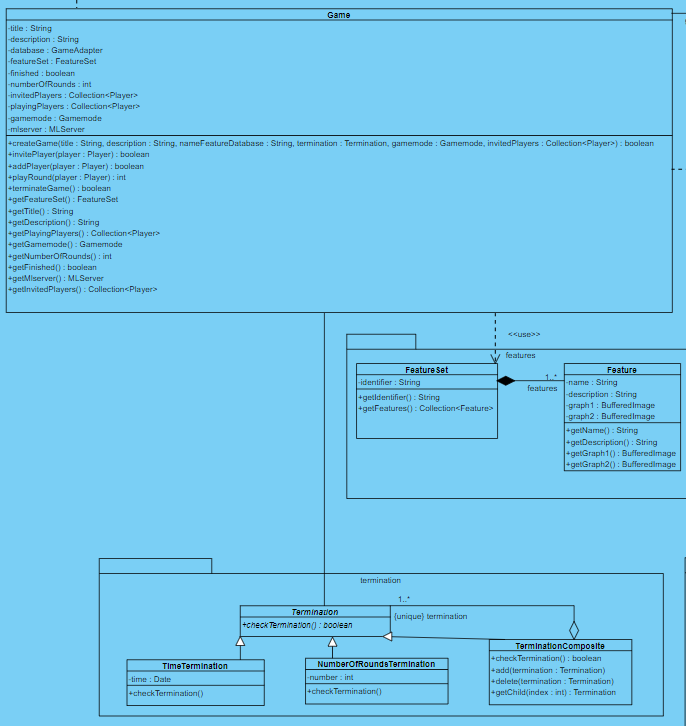
\includegraphics[width=\textwidth]{img/GameTerminationFeature.PNG}
	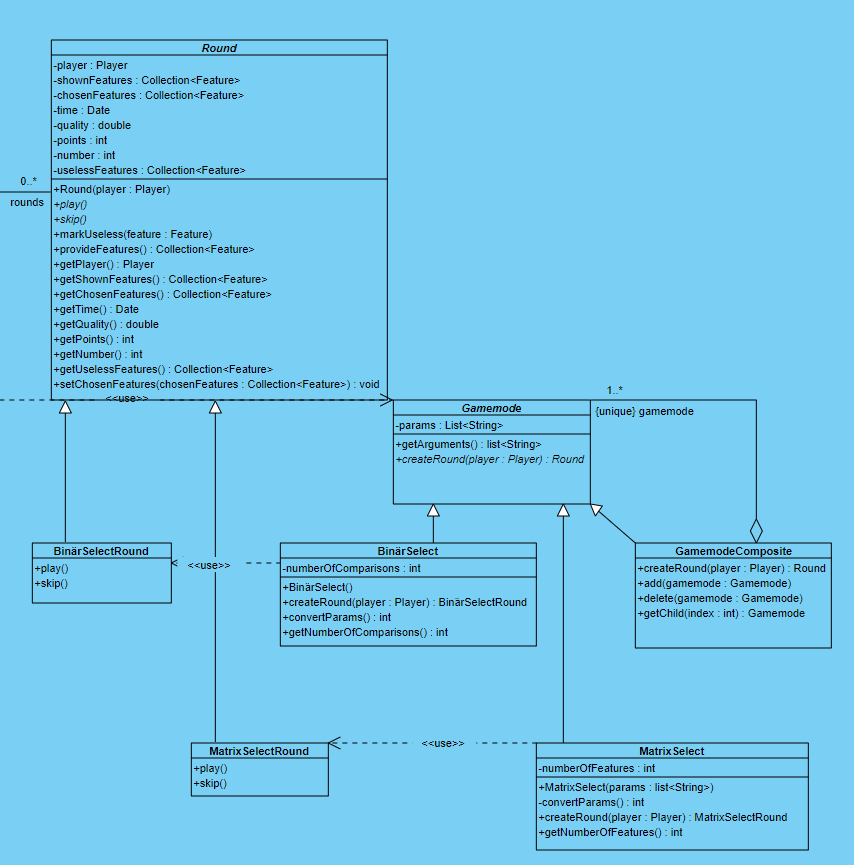
\includegraphics[width=\textwidth]{img/RoundAndGameMode.PNG}
	Paket, welches die innere Spielmechanik verwaltet. Dazu gehören die Spiele mit ihrer Erstellung und ihren Abbruchbedingungen, Spielmodi, Runden und Merkmale.

	\subsection{Game}
	Stellt ein Spiel dar, verwaltet eingeladene und spielende Spieler sowie die zum Spiel zugehörigen Informationen
	\subsubsection{Game}
	\begin{itemize}
	\item Beschreibung: Konstruktor, der ein Game-Objekt erzeugt, die Attribute außer ID, numberOfRounds und finished werden über die Setter initialisiert
	\item Parameter: id: Die eindeutige Spiel-ID
	\end{itemize}

	\subsubsection{getTitle}
	\begin{itemize}
		\item Beschreibung: Gibt den Spieltitel zurück
		\item Rückgabewert: Der Spieltitel
	\end{itemize}
	\subsubsection{getDescription}
	\begin{itemize}
		\item Beschreibung: Gibt die Spielbeschreibung zurück
		\item Rückgabewert: Die Spielbeschreibung
	\end{itemize}
	\subsubsection{getFinished}
			\begin{itemize}
				\item Beschreibung: Gibt zurück, ob das Spiel noch aktiv ist
				\item Rückgabewert: False, falls Spiel beendet wurde, sonst true
			\end{itemize}
	\subsubsection{getNumberOfRounds}
		\begin{itemize}
			\item Beschreibung: Gibt die Anzahl der bereits gespielten Runden insgesamt zurück
			\item Rückgabewert: Die Anzahl der gespielten Runden
		\end{itemize}
	\subsubsection{getID}
		\begin{itemize}
		\item Beschreibung: Gibt die ID des Spiels zurück
		\item Rückgabewert: Die ID
		\end{itemize}
	\subsubsection{getInvitedPlayers}
		\begin{itemize}
			\item Beschreibung: Gibt eine Aufzählung aller E-Mail-Adressen der Spieler zurück, die eingeladen sind, die Einladung aber noch nicht angenommen haben
			\item Rückgabewert: Die Aufzählung der E-Mail-Adressen der eingeladenen Spieler
		\end{itemize}
	\subsubsection{getAddressOrganiserDatabase}
			\begin{itemize}
			\item Beschreibung: Gibt die Adresse der zum Spiel gehörigen Datenbank zurück
			\item Rückgabewert: Die Adresse der zum Spiel gehörigen Datenbank
			\end{itemize}
	\subsubsection{getPlayingPlayers}
		\begin{itemize}
			\item Beschreibung: Gibt eine Aufzählung aller Spieler zurück, die die Einladung angenommen haben und Runden spielen können
			\item Rückgabewert: Die Aufzählung der spielenden Spieler
		\end{itemize}
	\subsubsection{getTermination}
	\begin{itemize}
		\item Beschreibung: Gibt die zum Spiel gehörige Abbruchbedingung zurück
		\item Rückgabewert: Die zum Spiel gehörige Abbruchbedingung
		\end{itemize}
	\subsubsection{getFeatureSet}
		\begin{itemize}
			\item Beschreibung: Gibt den zum Spiel gehörigen Merkmalsdatensatz zurück
			\item Rückgabewert: Der Merkmalsdatensatz
		\end{itemize}
	\subsubsection{getGamemode}
	\begin{itemize}
		\item Beschreibung: Gibt den zum Spiel gehörigen Spielmodus zurück
		\item Rückgabewert: Der Spielmodus
	\end{itemize}
	\subsubsection{getMlserver}
	\begin{itemize}
		\item Beschreibung: Gibt den ML-Server an, der die Merkmale bereitstellt und die Qualitätsberechnung durchführt
		\item Rückgabewert: Der ML-Server
	\end{itemize}
	\subsubsection{getRounds}
	\begin{itemize}
		\item Beschreibung: Gibt die bisher abgeschlossenen, zum Spiel gehörigen Runden zurück
		\item Rückgabewert: Die abgeschlossenen Runden
		\end{itemize}
	\subsubsection{setTitle}
		\begin{itemize}
		\item Beschreibung: Setzt den Spieltitel auf den angegebenen Wert
		\item Parameter: title: Der Spieltitel
		\end{itemize}
	\subsubsection{setDescription}
		\begin{itemize}
		\item Beschreibung: Setzt die Spielbeschreibung auf den angegebenen Wert
		\item Parameter: description: Die Spielbeschreibung
		\end{itemize}
	\subsubsection{setAddressOrganiserDatabase}
		\begin{itemize}
		\item Beschreibung: Speichert die Adresse der vom Organisator angegebene Datenbank als die zum Spiel gehörige, auf der die Spielinformationen gespeichert werden
		\item Parameter: addressOrganiserDatabase: Die Adresse der Datenbank, in die die Spielinformationen geschrieben werden
		\end{itemize}
	\subsubsection{setTermination}
		\begin{itemize}
		\item Beschreibung: Setzt die Abbruchbedingung, die bestimmt, wann das Spiel terminiert
		\item Parameter: termination: Die Abbruchbedingung des Spiels
		\end{itemize}
	\subsubsection{setFeatureSet}
				\begin{itemize}
				\item Beschreibung: Speichert den angegebenen Merkmalsdatensatz als den zum Spiel gehörigen
				\item Parameter: featureset: Der Merkmalsdatensatz, aus dem die im Spiel angezeigten Merkmale kommen
				\end{itemize}
	\subsubsection{setGamemode}
		\begin{itemize}
		\item Beschreibung: Setzt den Spielmodus des Spiels auf den angegebenen Spielmodus
		\item Parameter: gamemode: Der Spielmodus des Spiels
		\end{itemize}	
	\subsubsection{setMlserver}
		\begin{itemize}
		\item Beschreibung: Speichert den angegebenen ML-Server als den zum Spiel gehörigen
		\item Parameter: mlserver: Der ML-Server, von dem der Merkmalsdatensatz kommt und der die Bewertung durchführt
		\end{itemize}
	\subsubsection{invitePlayers}
		\begin{itemize}
			\item Beschreibung: Fügt dem Spiel Spieler hinzu, die eingeladen wurden
			\item Parameter: playerEmails: Die E-Mail-Adressen der eingeladenen Spieler
			\item Rückgabewert: Ob Spieler erfolgreich hinzugefügt wurden oder schon im Spiel vorhanden sind
		\end{itemize}
	\subsubsection{acceptInvite}
		\begin{itemize}
			\item Beschreibung: Gibt einem Spieler die Spielberechtigung, der eine Einladung erhalten und diese angenommen hat
			\item Parameter:
			\begin{itemize}
			\item player: Der Spieler, der die Einladung angenommen hat
			\item email: Die E-Mail-Adresse des Spielers
			\end{itemize}
			\item Rückgabewert: Ob Spieler erfolgreich hinzugefügt wurde oder entweder schon spielt oder keine Einladung hatte
		\end{itemize}
	\subsubsection{declineInvite}
		\begin{itemize}
			\item Beschreibung: Löscht die E-Mail-Adresse eines Spielers aus der Aufzählung der eingeladenen Spieler, der eine Einladung abgelehnt hat
			\item Parameter: playerEmail: E-Mail-Adresse des Spielers, der die Einladung abgelehnt hat
			\item Rückgabewert: False, falls der Spieler gar keine aktive Einladung hatte
		\end{itemize}
	\subsubsection{startRound}
		\begin{itemize}
			\item Beschreibung: Startet das Spielen einer Runde durch einen Spieler, erzeugt dafür ein Rundenobjekt, auf dem es die start-Methode aufruft und die anzuzeigenden Merkmale zurückbekommt und selbst zurückgibt
			\item Parameter: playerID: ID des Spielers, der die Runde spielt
			\item Rückgabewert: Die Merkmale, die dem Spieler insgesamt anzuzeigen sind
		\end{itemize}
	\subsubsection{terminateGame}
		\begin{itemize}
			\item Beschreibung: Beendet ein Spiel
			\item Rückgabewert: Ob das Spiel erfolgreich beendet wurde
		\end{itemize}
	\subsubsection{addFinishedRound}
	\begin{itemize}
	\item Beschreibung: Fügt eine Runde zu den abgeschlossenen Runden hinzu, sorgt dafür, dass diese in der angegebenen Datenbank gespeichert wird
	\item Parameter: round: Die abgeschlossene Runde
	\end{itemize}

	\subsection{FeatureSet}
	Stellt einen Merkmalsdatensatz dar, der aus beliebig vielen Merkmalen besteht und den Namen des Datensatzes auf dem ML-Server als eindeutigen Identifikationsschlüssel hat
	\subsubsection{FeatureSet}
		\begin{itemize}
		\item Beschreibung: Konstruktor, der ein FeatureSet-Objekt erzeugt
		\item Parameter: identifier: Der Identifikationsschlüssel des Merkmalsdatensatzes
		\end{itemize}
	\subsubsection{getIdentifier}
	\begin{itemize}
		\item Beschreibung: Gibt den eindeutigen Identifikationsschlüssel eines Merkmalsdatensatzes zurück
		\item Rückgabewert: Der Identifikationsschlüssel
	\end{itemize}
	\subsubsection{getFeatures}
	\begin{itemize}
		\item Beschreibung: Gibt die zum Merkmalsdatensatz gehörigen Merkmale zurück
		\item Rückgabewert: Aufzählung der Merkmale
	\end{itemize}
	\subsubsection{addFeature}
	\begin{itemize}
	\item Beschreibung: Fügt ein Merkmal zum Merkmalsdatensatz hinzu
	\item Parameter: feature: Das Merkmal, das hinzugefügt werden soll
	\end{itemize}
	
	\subsection{Feature}
	Stellt ein zu einem Merkmalsdatensatz gehöriges Merkmal dar
	\subsubsection{Feature}
		\begin{itemize}
		\item Beschreibung: Konstruktor, der ein Feature-Objekt erzeugt
		\item Parameter:
		\begin{itemize}
		\item id: Die ID des Merkmals
		\item internalName: Der vom ML-Server angegebene interne Name des Merkmals
		\end{itemize}
		\end{itemize}
	\subsubsection{getID}
			\begin{itemize}
				\item Beschreibung: Gibt die ID des Spiels zurück
				\item Rückgabewert: Die ID
			\end{itemize}
	\subsubsection{getInternalName}
		\begin{itemize}
			\item Beschreibung: Gibt den internen Namen des Merkmals zurück
			\item Rückgabewert: Der interne Name
		\end{itemize}
	\subsubsection{getGermanName}
	\begin{itemize}
		\item Beschreibung: Gibt den Namen des Merkmals auf Deutsch zurück
		\item Rückgabewert: Der deutsche Name
	\end{itemize}
	\subsubsection{getEnglishName}
		\begin{itemize}
			\item Beschreibung: Gibt den Namen des Merkmals auf Englisch zurück
			\item Rückgabewert: Der englische Name
		\end{itemize}
	\subsubsection{getGermanDescription}
	\begin{itemize}
		\item Beschreibung: Gibt die Beschreibung des Merkmals auf Deutsch zurück
		\item Rückgabewert: Die deutsche Beschreibung
	\end{itemize}
	\subsubsection{getEnglishDescription}
		\begin{itemize}
			\item Beschreibung: Gibt die Beschreibung des Merkmals auf Englisch zurück
			\item Rückgabewert: Die englische Beschreibung
		\end{itemize}
	\subsubsection{getTotalGraph}
	\begin{itemize}
		\item Beschreibung: Gibt den Graphen des Merkmals zurück, der die Daten insgesamt anzeigt
		\item Rückgabewert: Der Graph mit Gesamtdaten
	\end{itemize}
	\subsubsection{getClassGraph}
	\begin{itemize}
		\item Beschreibung: Gibt den Graphen des Merkmals zurück, der die Daten nach Klassen aufgeteilt anzeigt
		\item Rückgabewert: Der Graph mit den Klassendaten
	\end{itemize}
	\subsubsection{setGermanName}
	\begin{itemize}
	\item Beschreibung: Setzt den deutschen Namen auf den angegebenen String
	\item Parameter: Der deutsche Name
	\end{itemize}
	\subsubsection{setEnglishName}
		\begin{itemize}
		\item Beschreibung: Setzt den englischen Namen auf den angegebenen String
		\item Parameter: Der englische Name
		\end{itemize}
	\subsubsection{setGermanDescription}
		\begin{itemize}
		\item Beschreibung: Setzt die deutsche Beschreibung auf den angegebenen String
		\item Parameter: Die deutsche Beschreibung
		\end{itemize}
	\subsubsection{setEnglishDescription}
		\begin{itemize}
		\item Beschreibung: Setzt die englische Beschreibung auf den angegebenen String
		\item Parameter: Die englische Beschreibung
		\end{itemize}
	\subsubsection{setTotalGraph}
		\begin{itemize}
		\item Beschreibung: Speichert den gesamten Graphen
		\item Parameter: Der Gesamtgraph
		\end{itemize}
	\subsubsection{setClassGraph}
		\begin{itemize}
		\item Beschreibung: Speichert den Klassengraphen
		\item Parameter: Der Klassengraph
		\end{itemize}

	\subsection{Termination}
	Stellt eine Abbruchbedingung, die zu einem Spiel gehört, dar
	\subsubsection{checkTermination}
	\begin{itemize}
		\item Beschreibung: Überprüft, ob die Abbruchbedingung erfüllt ist und beendet gegebenenfalls das Spiel
		\item Rückgabewert: True, wenn Bedingung erfüllt war, false sonst
	\end{itemize}

	\subsection{TerminationComposite}
	Stellt ein Kompositum aus eindeutigen Abbruchbedingungen dar, um unterschiedliche Abbruchbedingungen für ein Spiel zuzulassen, eine spezielle Abbruchbedingung
	\subsubsection{TerminationComposite}
		\begin{itemize}
		\item Beschreibung: Konstruktor, der ein TerminationComposite-Objekt erzeugt
		\end{itemize}
	\subsubsection{checkTermination}
	\begin{itemize}
		\item Beschreibung: Implementiert checkTermination von Termination, in dem für jede zugehörige Abbruchbedingung diese Methode ausgeführt wird
	\end{itemize}
	\subsubsection{add}
	\begin{itemize}
		\item Beschreibung: Fügt eine Abbruchbedingung zum Kompositum hinzu
		\item Parameter: termination: die Abbruchbedingung
	\end{itemize}
	\subsubsection{delete}
	\begin{itemize}
		\item Beschreibung: Entfernt eine Abbruchbedingung aus dem Kompositum
		\item Parameter: termination: die zu entfernende Abbruchbedingung
	\end{itemize}


	\subsection{TimeTermination}
	Sorgt dafür, dass ein Spiel zu einer bestimmten Zeit terminiert
	\subsubsection{TimeTermination}
		\begin{itemize}
		\item Beschreibung: Konstruktor, der ein TimeTermination-Objekt erzeugt
		\item Parameter: time: Die Zeit, zu der das Spiel terminieren soll
		\end{itemize}
	\subsubsection{checkTermination}
	\begin{itemize}
		\item Beschreibung: Implementiert die Methode, in dem überprüft wird, ob die Zeit erreicht ist
	\end{itemize}

	\subsection{NumberOfRoundsTermination}
	Sorgt dafür, dass ein Spiel nach bestimmter Anzahl an gespielten Runden terminiert
	\subsubsection{NumberOfRoundsTermination}
		\begin{itemize}
		\item Beschreibung: Konstruktor, der ein NumberOfRoundsTermination-Objekt erzeugt
		\item Parameter: number: Die Anzahl an Runden, nach der das Spiel terminieren soll
		\end{itemize}
	\subsubsection{checkTermination}
	\begin{itemize}
		\item Beschreibung: Implementiert die Methode, in dem geprüft wird, ob die Rundenzahl erreicht ist
	\end{itemize}

	\subsection{Round}
	Stellt eine Verallgemeinerung einer konkreten Runde eines bestimmten Spiels dar, verwaltet die zugehörigen Informationen, abstrakt
	\subsubsection{Round}
		\begin{itemize}
		\item Beschreibung: Konstruktor, der ein Round-Objekt erzeugt
		\item Parameter:
		\begin{itemize}
		\item player: Der Spieler, der die Runde spielt
		\item numberOfRound: Die Zahl gibt an, die wievielte Runde des Spiels diese Runde ist
		\end{itemize}
		\end{itemize}
	\subsubsection{getShownFeatures}
	\begin{itemize}
		\item Beschreibung: Gibt die Merkmale zurück, die dem Spieler angezeigt werden
		\item Rückgabewert: Die angezeigten Merkmale
	\end{itemize}
	\subsubsection{getChosenFeatures}
	\begin{itemize}
		\item Beschreibung: Gibt die Merkmale zurück, die vom Spieler ausgewählt wurden
		\item Rückgabewert: Die ausgewählten Merkmale
	\end{itemize}
	\subsubsection{getTime}
	\begin{itemize}
		\item Beschreibung: Gibt den Zeitpunkt zurück, an dem die Runde gestartet wurde
		\item Rückgabewert: Der Startzeitpunkt
	\end{itemize}
	\subsubsection{getQuality}
	\begin{itemize}
		\item Beschreibung: Gibt die Bewertung der Merkmalsauswahl durch den ML-Server zurück
		\item Rückgabewert: Die Bewertung zwischen 0 und 1
	\end{itemize}
	\subsubsection{getPoints}
	\begin{itemize}
		\item Beschreibung: Gibt die Anzahl an Punkten zurück, die der Spieler durch die Runde dazubekommen hat
		\item Rückgabewert: Die Anzahl der Punkte der Runde
	\end{itemize}
	\subsubsection{getNumberOfRound}
	\begin{itemize}
		\item Beschreibung: Gibt zurück, die wievielte Runde des Spiels diese Runde war
		\item Rückgabewert: Die Nummer der Runde
	\end{itemize}
	\subsubsection{getUselessFeatures}
	\begin{itemize}
		\item Beschreibung: Gibt alle Merkmale zurück, die als unwichtig markiert wurden
		\item Rückgabewert: Die unwichtigen Merkmale
	\end{itemize}
	\subsubsection{getPlayer}
		\begin{itemize}
			\item Beschreibung: Gibt den Spieler zurück, der die Runde spielt
			\item Rückgabewert: Der Spieler
		\end{itemize}
	\subsubsection{start}
		\begin{itemize}
			\item Beschreibung: Startet Runde, stellt Merkmale für die GUI bereit und gibt diese zurück
			\item Rückgabewert: Alle Merkmale, die dem Spieler insgesamt in dieser Runde angezeigt werden sollen
		\end{itemize}
	\subsubsection{skip}
		\begin{itemize}
			\item Beschreibung: Beendet die Runde ohne Merkmalsauswahl durch den Spieler und fügt die Runde als abgeschlossene Runde beim Spiel hinzu
			\item Parameter: uselessFeatures: Die vom Spieler als unnötig ausgewählten Merkmale
		\end{itemize}
	\subsubsection{selectFeatures}
	\begin{itemize}
	\item Beschreibung: Nimmt die Auswahl des Spielers entgegen, lässt die Qualität durch den ML-Server und die Punktzahl durch das zum Spieler gehörigen Gamification-Objekt berechnen und sorgt dafür, dass die Runde in die Datenbank und das Spiel geschrieben wird, gibt die Punktzahl zurück
	\item Parameter:
	\begin{itemize}
	 \item selectedFeatures: Die vom Spieler ausgewählten Merkmale
	 \item uselessFeatures: Die vom Spieler als unnötig ausgewählten Merkmale
	 \end{itemize}
	\item Rückgabewert: Die mit der Merkmalsauswahl erreichte Punktzahl der Runde
	\end{itemize}
	\subsubsection{provideFeatures}
				\begin{itemize}
					\item Beschreibung: Abstrakt, wählt Merkmale aus dem zum Spiel gehörigen Merkmalen aus, die dem Spieler angezeigt werden sollen
					\item Rückgabewert: Die Aufzählung der Merkmale
				\end{itemize}

	\subsection{StandardRound}
	Fasst alle Runden zusammen, die sich nur anhand der Zahl ihrer Vergleiche, der angezeigten Merkmale oder der auszuwählenden Merkmale unterscheiden
	\subsubsection{StandardRound}
	\begin{itemize}
	\item Beschreibung: Konstruktor, der ein StandardRound-Objekt erzeugt
	\item Parameter: 
	\begin{itemize}
	\item player: Der Spieler, der die Runde spielt
	\item numberOfRound: Die Zahl gibt an, die wievielte Runde des Spiels diese Runde ist
	\item numberOfSelections: Die Anzahl an verschiedenen Merkmalsauswahlen pro Runde
	\item featuresPerSelection: Die Anzahl an Merkmalen, die pro Auswahl angezeigt werden sollen
	\item minSelect: Die Anzahl an Merkmalen, die pro Auswahl mindestens ausgewählt werden muss
	\item maxSelect: Die Anzahl an Merkmalen, die pro Auswahl maximal ausgewählt werden muss
	\end{itemize}
	\end{itemize}
	\subsubsection{getNumberOfSelections}
	\begin{itemize}
		\item Beschreibung: Gibt die Anzahl an Auswahlen pro Runde zurück
		\item Rückgabewert: Anzahl an Auswahlen
	\end{itemize}
	\subsubsection{getFeaturesPerSelection}
	\begin{itemize}
		\item Beschreibung: Gibt die Anzahl an Merkmalen zurück, die pro Auswahl angezeigt werden
		\item Rückgabewert: Anzahl an Merkmalen pro Auswahl
	\end{itemize}
	\subsubsection{getMinSelect}
	\begin{itemize}
		\item Beschreibung: Gibt die Anzahl an Merkmalen zurück, die pro Auswahl minimal ausgewählt werden müssen
		\item Rückgabewert: Die Anzahl an Merkmalen
	\end{itemize}
	\subsubsection{getMaxSelect}
	\begin{itemize}
		\item Beschreibung: Gibt die Anzahl an Merkmalen zurück, die pro Auswahl maximal ausgewählt werden müssen
		\item Rückgabewert: Die Anzahl an Merkmalen
	\end{itemize}
	\subsubsection{provideFeatures}
	\begin{itemize}
	\item Beschreibung: Wählt pro Vergleich die angegebene Anzahl an Merkmalen aus und gibt diese alle in einer Liste hintereinander zurück
	\end{itemize}

	\subsection{Gamemode}
	Stellt einen Spielmodus dar, fungiert als Fabrik für die Runden
	\subsubsection{createRound}
	\begin{itemize}
		\item Beschreibung: Erzeugt eine Runde des Spielmodus
		\item Rückgabewert: Die erzeugte Runde
	\end{itemize}

	\subsection{GamemodeComposite}
	Kompositum aus verschiedenen Spielmodi, um zu ermöglichen, dass mehrere Spielmodi ausgewählt werden können
	\subsubsection{GamemodeComposite}
		\begin{itemize}
		\item Beschreibung: Konstruktor, der ein GamemodeComposite-Objekt erzeugt
		\end{itemize}
	\subsubsection{createRound}
	\begin{itemize}
		\item Beschreibung: Erzeugt eine Runde eines zufälligen Spielmodus des Kompositums
	\end{itemize}
	\subsubsection{add}
	\begin{itemize}
		\item Beschreibung: Fügt einen Spielmodus zum Kompositum hinzu
		\item Parameter: gamemode: der Spielmodus
	\end{itemize}
	\subsubsection{delete}
	\begin{itemize}
		\item Beschreibung: Entfernt einen Spielmodus aus dem Kompositum
		\item Parameter: gamemode: der zu entfernende Spielmodus
	\end{itemize}

	\subsection{BinärSelect}
	Stellt den Spielmodus BinärSelect dar, dessen Runden standardmäßig aufgebaut sind, also werden StandardRounds erzeugt
	\subsubsection{BinärSelect}
		\begin{itemize}
		\item Beschreibung: Konstruktor, der ein BinärSelect-Objekt erzeugt
		\end{itemize}
	\subsubsection{createRound}
	\begin{itemize}
		\item Beschreibung: Erzeugt eine Runde des Spielmodus BinärSelect, also eine StandardRound mit 5 Vergleichen und 2 Merkmalen pro Vergleich, von denen genau eines ausgewählt werden muss
	\end{itemize}

	\subsection{MatrixSelect}
	Stellt den Spielmodus MatrixSelect dar, dessen Runden standardmäßig aufgebaut sind, also werden StandardRounds erzeugt
	\subsubsection{MatrixSelect}
		\begin{itemize}
		\item Beschreibung: Konstruktor, der ein MatrixSelect-Objekt erzeugt
		\item Parameter:
		\begin{itemize}
		\item numberOfFeatures: Die Anzahl an Merkmalen, die pro Runde angezeigt werden müssen
		\item minSelect: Die Anzahl an Merkmalen, die pro Runde mindestens ausgewählt werden müssen
		\item maxSelect: Die Anzahl an Merkmalen, die pro Runde maximal ausgewählt werden müssen
		\end{itemize}
		\end{itemize}
	\subsubsection{createRound}
	\begin{itemize}
		\item Beschreibung: Erzeugt eine Runde des Spielmodus MatrixSelect, also eine StandardRound, setzt die Anzahl an Merkmalen pro Runde und die Anzahl an minimal und maximal auszuwählenden Merkmalen so wie die Attribute des Spielmodus belegt sind sowie die Anzahl an Merkmalsauswahlen auf 1
	\end{itemize}


	\section{Gamification}
	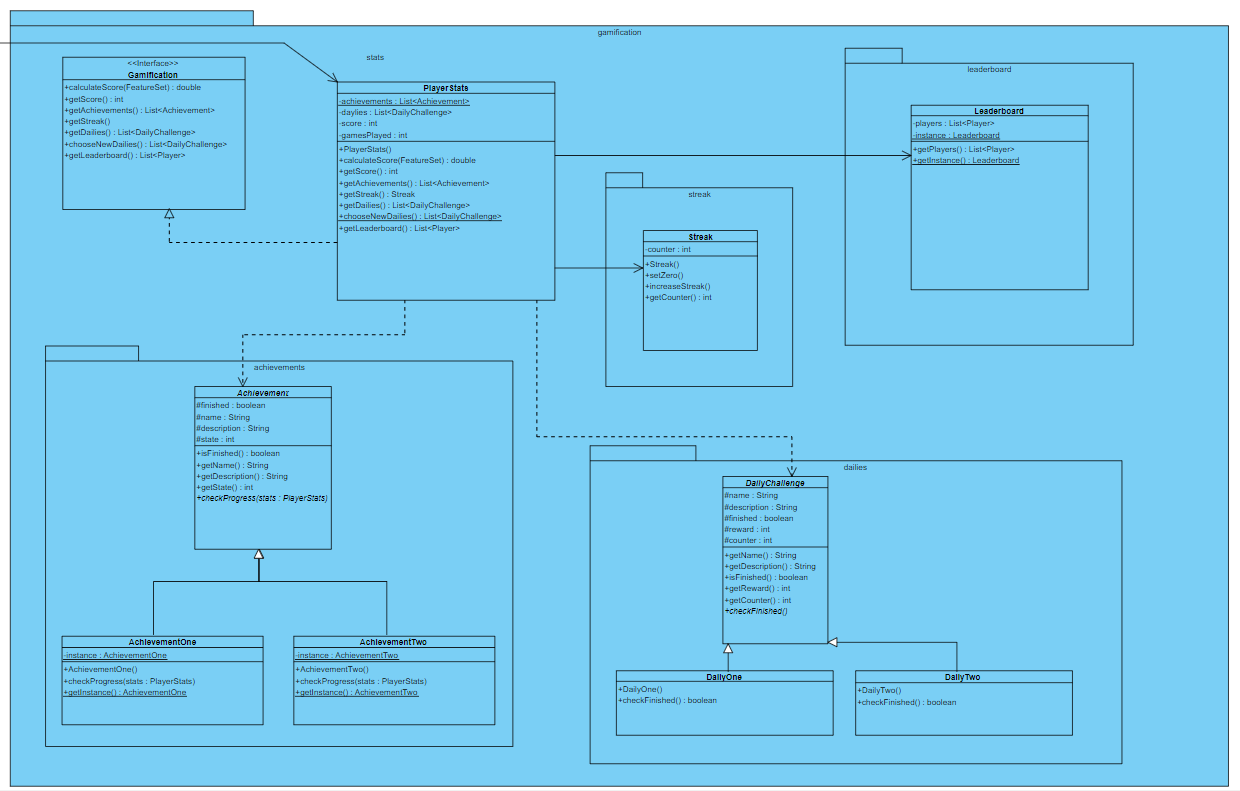
\includegraphics[width=\textwidth]{img/Gamification.PNG}\\
	Paket für die Gamification-Elemente. \\
	Zu den Gamification-Elementen gehören Punkte, Streak, Leaderboard, Achievements und Daily-Challenges.


	\subsection{Streak}
	Stellt eine Streak dar.

	\subsubsection{Streak}
	\begin{itemize}
		\item Beschreibung: Der Konstruktor einer Streak initialisiert den Zähler der Streak mit 0.
	\end{itemize}
	\subsubsection{setZero}
	\begin{itemize}
		\item Beschreibung: Setzt den Zähler der Streak auf den Wert 0 zurück.
	\end{itemize}
	\subsubsection{increaseStreak}
	\begin{itemize}
		\item Beschreibung: Erhöht den Zähler der Streak um den Wert 1.
	\end{itemize}
	\subsubsection{getCounter}
	\begin{itemize}
		\item Beschreibung: Gibt den aktuellen Zähler zurück.
		\item Rückgabewert: Der aktuelle Wert des Zählers.
	\end{itemize}


	\subsection{Leaderboard}
	Stellt ein Leaderboard dar. Es enthält eine Liste von Spielern. \\
	Hierfür wird das Singleton-Entwurfsmuster verwendet, damit nur ein Leaderboard-Objekt existiert.

	\subsubsection{Leaderboard}
	\begin{itemize}
		\item Beschreibung: Privater Konstruktor, der noch nichts initialisiert.
	\end{itemize}
	\subsubsection{getPlayers}
	\begin{itemize}
		\item Beschreibung: Gibt eine Liste von allen registrierten Spielern zurück. Diese ist nach der ausgewählten Sortierung der Spieler sortiert.
		\item Rückgabewert: Sortierte Liste von Spielern.
	\end{itemize}
	\subsubsection{getInstance}
	\begin{itemize}
		\item Beschreibung: Statische Methode. Sorgt dafür, dass nur ein Leaderboard-Objekt existiert und gibt dieses zurück.
		\item Rückgabewert: Das Leaderboard-Objekt.
	\end{itemize}
	\subsubsection{setSortingStrategy}
	\begin{itemize}
		\item Beschreibung: Setzt die Strategie, nach der die Liste an Spielern sortiert werden soll.
		\item Parameter: Die gewünschte Sortierungsstrategie.
	\end{itemize}

	\subsection{LeaderboardSortingStrategy}
	Eine abstrakte Klasse für die verschiedenen Sortierungen des Leaderboards. Jede Unterklasse muss die Methode sort implementieren.
	\subsubsection{sort}
	\begin{itemize}
		\item Beschreibung: Sortiert die Liste des Leaderboards nach bestimmten Kriterien.
		\item Parameter: Die zu sortierende Liste von Spielern.
	\end{itemize}

	\subsection{SortScoreAllTime}
	Erbt von der Klasse LeaderboardSortingStrategy. Bietet eine Sortierung an, die nach Gesamtpunktzahlen der Spieler über den gesamten Zeitraum sortiert.
	\subsubsection{sort}
	\begin{itemize}
		\item Beschreibung: Sortiert die Liste des Leaderboards nach den Gesamtpunktzahlen der Spieler.
		\item Parameter: Die zu sortierende Liste von Spielern.
	\end{itemize}

	\subsection{SortScoreLastWeek}
	Erbt von der Klasse LeaderboardSortingStrategy. Bietet eine Sortierung an, die nach Gesamtpunktzahlen der Spieler, welche in der letzten Woche erreicht wurden, sortiert.
	\subsubsection{sort}
	\begin{itemize}
		\item Beschreibung: Sortiert die Liste des Leaderboards nach den erreichten Punkten der letzten sieben Tage der Spieler.
	\end{itemize}


	\subsection{DailyChallenge}
	Die abstrakte Klasse DailyChallenge gibt an, wie konkrete Daily-Challenges aufgebaut sind. Die Methoden checkFinished und resetDaily sind abstrakt und müssen von den Unterklassen implementiert werden. \\

	\subsubsection{getName}
	\begin{itemize}
		\item Beschreibung: Gibt den Namen der Daily-Challenge zurück.
		\item Rückgabewert: Ein String vom Namen der Daily-Challenge.
	\end{itemize}
	\subsubsection{getDescription}
	\begin{itemize}
		\item Beschreibung: Gibt die Beschreibung der Daily-Challenge zurück.
		\item Rückgabewert: Ein String von der Beschreibung der Daily-Challenge.
	\end{itemize}
	\subsubsection{getDate}
	\begin{itemize}
		\item Beschreibung: Gibt das Datum\footnote{Für das Datum wird die Java Bibliothek java.util.Date benutzt.} der Daily-Challenge zurück.
		\item Rückgabewert: Das Datum der Daily-Challenge.
	\end{itemize}
	\subsubsection{setDate}
	\begin{itemize}
		\item Beschreibung: Setzt das Datum der Daily-Challenge.
		\item Parameter: Das Datum der Daily-Challenge.
	\end{itemize}
	\subsubsection{isCompleted}
	\begin{itemize}
		\item Beschreibung: Überprüft, ob die Aufgabe der Daily-Challenge an einem Tag schon erfüllt wurde.
		\item Rückgabewert: True, wenn die Aufgabe schon erfüllt ist, sonst false.
	\end{itemize}
	\subsubsection{getReward}
	\begin{itemize}
		\item Beschreibung: Gibt eine Punktzahl, die als Belohnung für das Abschließen einer Daily-Challenge fungiert, zurück.
		\item Rückgabewert: Eine Punktzahl, die die Belohnung darstellt.
	\end{itemize}
	\subsubsection{resetDaily}
	\begin{itemize}
		\item Beschreibung: Setzt die Werte der Daily-Challenge wieder auf ihren Anfangswert zurück.
	\end{itemize}
	\subsubsection{checkFinished}
	\begin{itemize}
		\item Beschreibung: Überprüft, ob die Aufgabe der Daily-Challenge erfüllt ist.
		\item Parameter: Das zugehörige PlayerStats-Objekt eines Spielers.
		\item Rückgabewert: True, wenn die Aufgabe erfüllt ist, sonst false.
	\end{itemize}

	\subsection{DailyPlayThreeRounds}
	Konkrete Implementierung der abstrakten Klasse DailyChallenge, in der der Spieler drei Runden an einem Tag spielen muss, um sie abzuschließen.
	\subsubsection{DailyPlayThreeRounds}
	\begin{itemize}
		\item Beschreibung: Der Konstruktor von DailyPlayThreeRounds setzt Namen und Beschreibung von DailyPlayThreeRounds sowie die Belohnung. Der Runden-Zähler werden auf 0 gesetzt und completed auf false.
	\end{itemize}
	\subsubsection{checkFinished}
	\begin{itemize}
		\item Beschreibung: Überprüft, ob der Spieler schon drei Runden an diesem Tag gespielt hat.
		\item Parameter: Das zugehörige PlayerStats-Objekt eines Spielers.
		\item Rückgabewert: True, wenn der Spieler schon drei Runden an diesem Tag gespielt hat. False, falls er die Aufgabe der Daily-Challenge schon erreicht hat oder sie noch nicht erfüllt hat.
	\end{itemize}
	\subsubsection{resetDaily}
	\begin{itemize}
		\item Beschreibung: Setzt den Runden-Zähler auf 0 und das Attribut completed auf false.
	\end{itemize}
	\subsubsection{getRoundsPlayed}
	\begin{itemize}
		\item Beschreibung: Gibt den Runden-Zähler der Daily-Challenge zurück.
		\item Rückgabewert: Die Anzahl der am heutigen Tag gespielten Runden.
	\end{itemize}

	\subsection{DailyGetStreakThree}
	Konkrete Implementierung der abstrakten Klasse DailyChallenge, in der der Spieler eine 3er-Streak, also drei Runden hintereinander gespielt haben muss, um sie abzuschließen.
	\subsubsection{DailyGetStreakOfThree}
	\begin{itemize}
		\item Beschreibung: Der Konstruktor von DailyGetStreakThree setzt Namen und Beschreibung von DailyGetStreakThree sowie die Belohnung. Der Streak-Zähler werden auf 0 gesetzt und completed auf false.
	\end{itemize}
	\subsubsection{checkFinished}
	\begin{itemize}
		\item Beschreibung: Überprüft, ob der Spieler schon eine Streak in Höhe von drei an diesem Tag erreicht hat.
		\item Parameter: Das zugehörige PlayerStats-Objekt eines Spielers.
		\item Rückgabewert: True, wenn der Spieler schon eine Streak in Höhe von drei an diesem Tag erreicht hat. False, falls er die Aufgabe der Daily-Challenge schon erreicht hat oder sie noch nicht erfüllt hat.
	\end{itemize}
	\subsubsection{resetDaily}
	\begin{itemize}
		\item Beschreibung: Setzt den Streak-Zähler auf 0 und das Attribut completed auf false.
	\end{itemize}
	\subsubsection{getStreak}
	\begin{itemize}
		\item Beschreibung: Gibt den Streak-Zähler der Daily-Challenge zurück.
		\item Rückgabewert: Die Höhe der momentanen Streak vom heutigen Tag.
	\end{itemize}

	\subsection{DailyReachScoreHundredFifty}
	Konkrete Implementierung der abstrakten Klasse DailyChallenge, in der der Spieler 150 Punkte an einem Tag erreichen muss.
	\subsubsection{DailyReachScoreHundredFifty}
	\begin{itemize}
		\item Beschreibung: Der Konstruktor von DailyReachScoreHundred setzt Namen und Beschreibung von DailyReachScoreHundred sowie die Belohnung. Der Punkte-Zähler werden auf 0 gesetzt und completed auf false.
	\end{itemize}
	\subsubsection{checkFinished}
	\begin{itemize}
		\item Beschreibung: Überprüft, ob der Spieler schon 150 Punkte an diesem Tag erreicht hat.
		\item Parameter: Das zugehörige PlayerStats-Objekt eines Spielers.
		\item Rückgabewert: True, wenn der Spieler schon 150 Punkte an diesem Tag erreicht hat. False, falls er die Aufgabe der Daily-Challenge schon erreicht hat oder sie noch nicht erfüllt hat.
	\end{itemize}
	\subsubsection{resetDaily}
	\begin{itemize}
		\item Beschreibung: Setzt den Punkte-Zähler auf 0 und das Attribut completed auf false.
	\end{itemize}
	\subsubsection{getScore}
	\begin{itemize}
		\item Beschreibung: Gibt den Punkte-Zähler der Daily-Challenge zurück.
		\item Rückgabewert: Die Höhe der momentanen erreichten Punkte am heutigen Tag.
	\end{itemize}

	\vspace{8pt}

	Diese drei konkreten Daily-Challenges sind bereits dem Entwurfsdiagramm zu entnehmen. Weitere Daily-Challenges werden analog hinzugefügt. Für eine Liste der vollständigen Daily-Challenges siehe \hyperlink{Daily}{Kapitel 8.2}. \\

	\vspace{8pt}

	\subsection{Achievement}
	Die abstrakte Klasse Achievement gibt an, wie konkrete Achievements aufgebaut sind. Lediglich die Methode checkProgress ist abstrakt und muss von den Unterklassen implementiert werden.

	\subsubsection{getName}
	\begin{itemize}
		\item Beschreibung: Gibt den Namen des Achievements zurück.
		\item Rückgabewert: Ein String vom Namen des Achievements.
	\end{itemize}
	\subsubsection{getDescription}
	\begin{itemize}
		\item Beschreibung: Gibt die Beschreibung des Achievements zurück.
		\item Rückgabewert: Ein String von der Beschreibung des Achievements.
	\end{itemize}
	\subsubsection{checkProgress}
	\begin{itemize}
		\item Beschreibung: Überprüft, wie weit die Aufgabe des Achievements erfüllt ist und setzt dementsprechend den Zustand des Achievements.
		\item Parameter: Das zugehörige PlayerStats-Objekt eines Spielers.
		\item Rückgabewert: Der entsprechende Zustand des Achievements.
	\end{itemize}

	\subsection{AchievementType}
	Ein Enum, welches die verschiedenen Zustände eines Achievements darstellt.

	\begin{itemize}
		\item INVISIBLE: Das Achievement soll noch nicht sichtbar sein.
		\item CONCEALED: Das Achievement ist sichtbar, aber es noch nicht erkenntlich, was getan werden muss, um es abzuschließen.
		\item SHOWN: Das Achievement ist angezeigt und man kennt die Abschlussbedingungen.
		\item FINISHED: Das Achievement ist beendet, das heißt, dass die Aufgabe des Achievements abgeschlossen wurde.
	\end{itemize}

	\subsection{AchievementPlayRounds}
	Eine abstrakte Klasse für Achievements von der Art, dass ein Spieler eine bestimmte Anzahl an Runden spielen muss, um es zu erreichen. Die Unterklassen müssen die abstrakte Methode checkProgress entsprechend implementieren.

	\subsection{AchievementGetStreak}
	Eine abstrakte Klasse für Achievements von der Art, dass ein Spieler eine bestimmte Streak erhalten muss, um es zu erreichen. Die Unterklassen müssen die abstrakte Methode checkProgress entsprechend implementieren.

	\subsection{AchievementCompleteDaily}
	Eine abstrakte Klasse für Achievements von der Art, dass ein Spieler eine bestimmte Anzahl an Daily-Challenges abschließen muss, um es zu erreichen. Die Unterklassen müssen die abstrakte Methode checkProgress entsprechend implementieren.

	\subsection{AchievementReachScore}
	Eine abstrakte Klasse für Achievements von der Art, dass ein Spieler eine bestimmte Punktzahl an Punkten erspielen muss, um es zu erreichen. Die Unterklassen müssen die abstrakte Methode checkProgress entsprechend implementieren.

	\subsection{AchievementReachTotalScoreHundred}
	Dieses konkrete Achievement erhält ein Spieler, wenn er eine Gesamtpunktzahl von mindestens 100 Punkten erreicht. Hierfür wird das Singleton-Entwurfsmuster verwendet, damit nur ein AchievementReachTotalScoreHundred-Objekt existiert.

	\subsubsection{AchievementReachTotalScoreHundred}
	\begin{itemize}
		\item Beschreibung: Der Konstruktor von AchievementReachTotalScoreHundred setzt Namen und Beschreibung von AchievementReachTotalScoreHundred.
	\end{itemize}
	\subsubsection{checkProgress}
	\begin{itemize}
		\item Beschreibung: Überprüft, wie weit die Aufgabe des Achievements erfüllt ist und setzt dementsprechend den Zustand des Achievements.
		\item Parameter: Das zugehörige PlayerStats-Objekt eines Spielers.
		\item Rückgabewert: Das Achievement hat immer den Zustand SHOWN, es sei denn es wurde erfüllt, dann hat es den Zustand FINISHED.
	\end{itemize}
	\subsubsection{getInstance}
	\begin{itemize}
		\item Beschreibung: Statische Methode. Sorgt dafür, dass nur ein AchievementReachTotalScoreHundred-Objekt existiert und gibt dieses zurück.
		\item Rückgabewert: Das AchievementReachTotalScoreHundred-Objekt.
	\end{itemize}

	\subsection{AchievementReachTotalScoreThousand}
	Dieses konkrete Achievement erhält ein Spieler, wenn er eine Gesamtpunktzahl von mindestens 1000 Punkten erreicht. Hierfür wird das Singleton-Entwurfsmuster verwendet, damit nur ein Leaderboard-Objekt existiert.

	\subsubsection{AchievementReachTotalScoreThousand}
	\begin{itemize}
		\item Beschreibung: Der Konstruktor von AchievementReachTotalScoreThousand setzt Namen und Beschreibung von AchievementReachTotalScoreThousand.
	\end{itemize}
	\subsubsection{checkProgress}
	\begin{itemize}
		\item Beschreibung: Überprüft, wie weit die Aufgabe des Achievements erfüllt ist und setzt dementsprechend den Zustand des Achievements.
		\item Parameter: Das zugehörige PlayerStats-Objekt eines Spielers.
		\item Rückgabewert: Das Achievement hat zunächst den Zustand CONCEALED, wenn der Spieler 500 Punkte erreicht wechselt es in den Zustand SHOWN und wenn der Spieler mindestens 1000 Punkte hat ist es im Zustand FINISHED.
	\end{itemize}
	\subsubsection{getInstance}
	\begin{itemize}
		\item Beschreibung: Statische Methode. Sorgt dafür, dass nur ein AchievementReachTotalScoreThousand-Objekt existiert und gibt dieses zurück.
		\item Rückgabewert: Das AchievementReachTotalScoreThousand-Objekt.
	\end{itemize}

	\vspace{8pt}

	Diese vier Achievement-Typen und zwei konkreten Achievements sind bereits dem Entwurfsdiagramm zu entnehmen. Weitere Achievement-Typen und konkrete Achievements werden analog hinzugefügt. Für eine Liste der vollständigen Achievements siehe \hyperlink{Ach}{Abschnitt 8.1}. \\

	\vspace{8pt}


	\subsection{Gamification}
	Die Schnittstelle Gamification abstrahiert von der konkreten Implementierung von Gamification-Elementen und gibt dabei zu implementierende Methoden vor. \\

	\subsubsection{calculateScore}
	\begin{itemize}
		\item Beschreibung: Berechnet aus gegebenem Wert eine entsprechende Punktzahl für den Spieler.
		\item Parameter: Double, ein Wert zwischen 0 und 1.
		\item Rückgabewert: Die berechnete erreichte Punktzahl des Spielers, eine ganze Zahl zwischen 0 und 100.
	\end{itemize}
	\subsubsection{skipRound}
	\begin{itemize}
		\item Beschreibung: Wenn der Spieler eine Runde überspringt, werden die nötigen Statistiken (Streaks) angepasst.
	\end{itemize}
	\subsubsection{getScore}
	\begin{itemize}
		\item Beschreibung: Gibt die aktuelle Punktzahl des Spielers zurück.
		\item Rückgabewert: Die aktuelle Punktzahl des Spielers.
	\end{itemize}
	\subsubsection{getAchievements}
	\begin{itemize}
		\item Beschreibung: Gibt die aktuelle Liste Achievements zurück.
		\item Rückgabewert: Die aktuelle Achievements des Spielers in einer Liste.
	\end{itemize}
	\subsubsection{getStreak}
	\begin{itemize}
		\item Beschreibung: Gibt die aktuelle Streak des Spielers zurück.
		\item Rückgabewert: Das Streak-Objekt des Spielers.
	\end{itemize}
	\subsubsection{getDaily}
	\begin{itemize}
		\item Beschreibung: Gibt die aktive Daily-Challenge des Spielers zurück.
		\item Rückgabewert: Das aktive Daily-Challenge-Objekt.
	\end{itemize}



	\subsection{PlayerStats}
	Die Klasse PlayerStats implementiert die Schnittstelle Gamification und regelt das Zusammenwirken der Gamification-Elemente und berechnet dabei die Punkte eines Spielers.

	\subsubsection{PlayerStats}
	Der Konstruktor von PlayerStats initialisiert die einzelnen Zähler mit dem Wert 0 und lädt sich die verfügbaren Achievements und Daily-Challenges.
	\subsection{getRoundsPlayed}
	\begin{itemize}
		\item Beschreibung: Gibt die Anzahl der gespielten Runden eines Spielers zurück.
		\item Rückgabewert: Die Anzahl der gespielten Runden.
	\end{itemize}
	\subsection{getDailiesCompleted}
	\begin{itemize}
		\item Beschreibung: Gibt die Anzahl der abgeschlossenen Daily-Challenges eines Spielers zurück.
		\item Rückgabewert: Die Anzahl der abgeschlossenen Daily-Challenges.
	\end{itemize}
	\subsection{getMaxRoundScore}
	\begin{itemize}
		\item Beschreibung: Gibt die höchste erzielte Punktzahl nach einer einzelnen Runde zurück (ohne Miteinbeziehung von Streaks).
		\item Rückgabewert: Die höchste erzielte Punktzahl nach einer einzelnen Runde.
	\end{itemize}
	\subsection{getLastScore}
	\begin{itemize}
		\item Beschreibung: Gibt die Punktzahl zurück, die in der letzten Runde erzielt wurde (ohne Miteinbeziehung von Streaks).
		\item Rückgabewert: Die Punktzahl der letzten Runde.
	\end{itemize}
	\subsection{getHighestStreak}
	\begin{itemize}
		\item Beschreibung: Gibt den Wert der höchsten Streak eines Spielers zurück.
		\item Rückgabewert: Den Wert der höchsten Streak.
	\end{itemize}




	\chapter{Front-End}
	Es wird pro Art der Seite eine Hauptseite geben, die dann über die REST-API mit nutzerspezifischen Inhalten gefüllt werden. \\
	Die Hauptseiten sind die folgenden: \\
	\begin{itemize}
		\item   Anmeldung
		\item   Organisator-Übersicht
		\item   Spielerstellung
		\item   Spieler-Übersicht
		\item   Spiel
	\end{itemize}
	%TODO Ich würde hier zu jedem Punkt evt. paar Sätze verlieren?


	\chapter{Sequenzdiagramme}

	\section{Organisation}
	\subsection{Nutzer anmelden}
	Das folgende Sequenzdiagramm korrespondiert zu Testszenario 8.1.2 (Spieler anmelden) und 8.1.5 (Organisator anmelden) aus dem Pflichtenheft.

	\subsection{Nutzer abmelden}
	Das folgende Sequenzdiagramm korrespondiert zu Testszenario 8.1.3 (Spieler abmelden) und 8.1.6 (Organisator abmelden) aus dem Pflichtenheft.

	\subsection{Organisator registrieren}
	Das folgende Sequenzdiagramm korrespondiert zu Testszenario 8.1.6. aus dem Pflichtenheft.

	\subsection{Spieler registrieren}
	Das folgende Sequenzdiagramm korrespondiert zu Testszenario 8.1.1. aus dem Pflichtenheft.

	\subsection{Spiel erstellen}
	Das folgende Sequenzdiagramm korrespondiert zu Testszenario 8.1.8. aus dem Pflichtenheft.

	\subsection{Spiel vorzeitig beenden}
	Das folgende Sequenzdiagramm korrespondiert zu Testszenario 8.1.10 aus dem Pflichtenheft.

	\subsection{Spiel löschen}
	Das folgende Sequenzdiagramm korrespondiert zu Testszenario 8.1.11 aus dem Pflichtenheft.

	\subsection{Spieleinstellungen speichern}
	Das folgende Sequenzdiagramm korrespondiert zu Testszenario 8.1.12 aus dem Pflichtenheft.

	\subsection{Spieleinstellungen laden}
	Das folgende Sequenzdiagramm korrespondiert zu Testszenario 8.1.13 aus dem Pflichtenheft.


	\section{Spiel}
	\subsection{Spieler einladen}
	Das folgende Sequenzdiagramm korrespondiert zu Testszenario 8.1.9 aus dem Pflichtenheft.

	\subsection{Einladung annehmen}
	Das folgende Sequenzdiagramm korrespondiert zu Testszenario 8.2.1 aus dem Pflichtenheft.

	\subsection{Einladung ablehnen}

	\subsection{Runde spielen, Merkmal als unwichtig markieren}
	Das folgende Sequenzdiagramm korrespondiert zu Testszenario 8.2.6. aus dem Pflichtenheft.

	\subsection{Runde überspringen}
	Das folgende Sequenzdiagramm korrespondiert zu Testszenario 8.2.5 aus dem Pflichtenheft.

	\subsection{Runde starten}
	Das folgende Sequenzdiagramm korrespondiert zu Testszenario 8.3.1. aus dem Pflichtenheft.

	\section{Gamification}
	\subsection{Achievements ansehen}
	Das folgende Sequenzdiagramm korrespondiert zu Testszenario 8.3.2. aus dem Pflichtenheft. \\


	\subsection{Leaderboard ansehen}
	Das folgende Sequenzdiagramm korrespondiert zu Testszenario 8.3.3. aus dem Pflichtenheft. \\


	\subsection{Streak erreichen}
	Das folgende Sequenzdiagramm korrespondiert zu Testszenario 8.2.7. aus dem Pflichtenheft. \\
	Es handelt sich hierbei um einen Ausschnitt von Sequenzdiagramm \enquote{Runde spielen, Merkmal als unwichtig markieren}. Es sind die relevanten Aufrufe zu sehen, welche die Streak eines Spielers erhöhen und ihm, wenn die Streak hoch genug, doppelte Punkte geben. \\

	\subsection{Daily-Challenge abschließen}
	Es handelt sich hierbei um einen Ausschnitt von Sequenzdiagramm \enquote{Runde spielen, Merkmal als unwichtig markieren}. Es sind die relevanten Aufrufe zu sehen, welche überprüfen, ob eine Daily-Challenge abgeschlossen wurde. \\


	\section{Administration}
	\subsection{Sprache ändern}
	Das folgende Sequenzdiagramm korrespondiert zu Testszenario 8.4.1 aus dem Pflichtenheft.

	\subsection{Passwort ändern}
	Das folgende Sequenzdiagramm korrespondiert zu Testszenario 8.4.4 aus dem Pflichtenheft.

	\subsection{E-Mail ändern}
	Das folgende Sequenzdiagramm korrespondiert zu Testszenario 8.4.5 aus dem Pflichtenheft.

	\subsection{Passwort zurücksetzen}
	Das folgende Sequenzdiagramm korrespondiert zu Testszenario 8.4.6 aus dem Pflichtenheft.






	\chapter{Zustandsdiagramme}
	\section{Streak}
	\hypertarget{StreakState}{}
	\label{fig:Streak_State}
	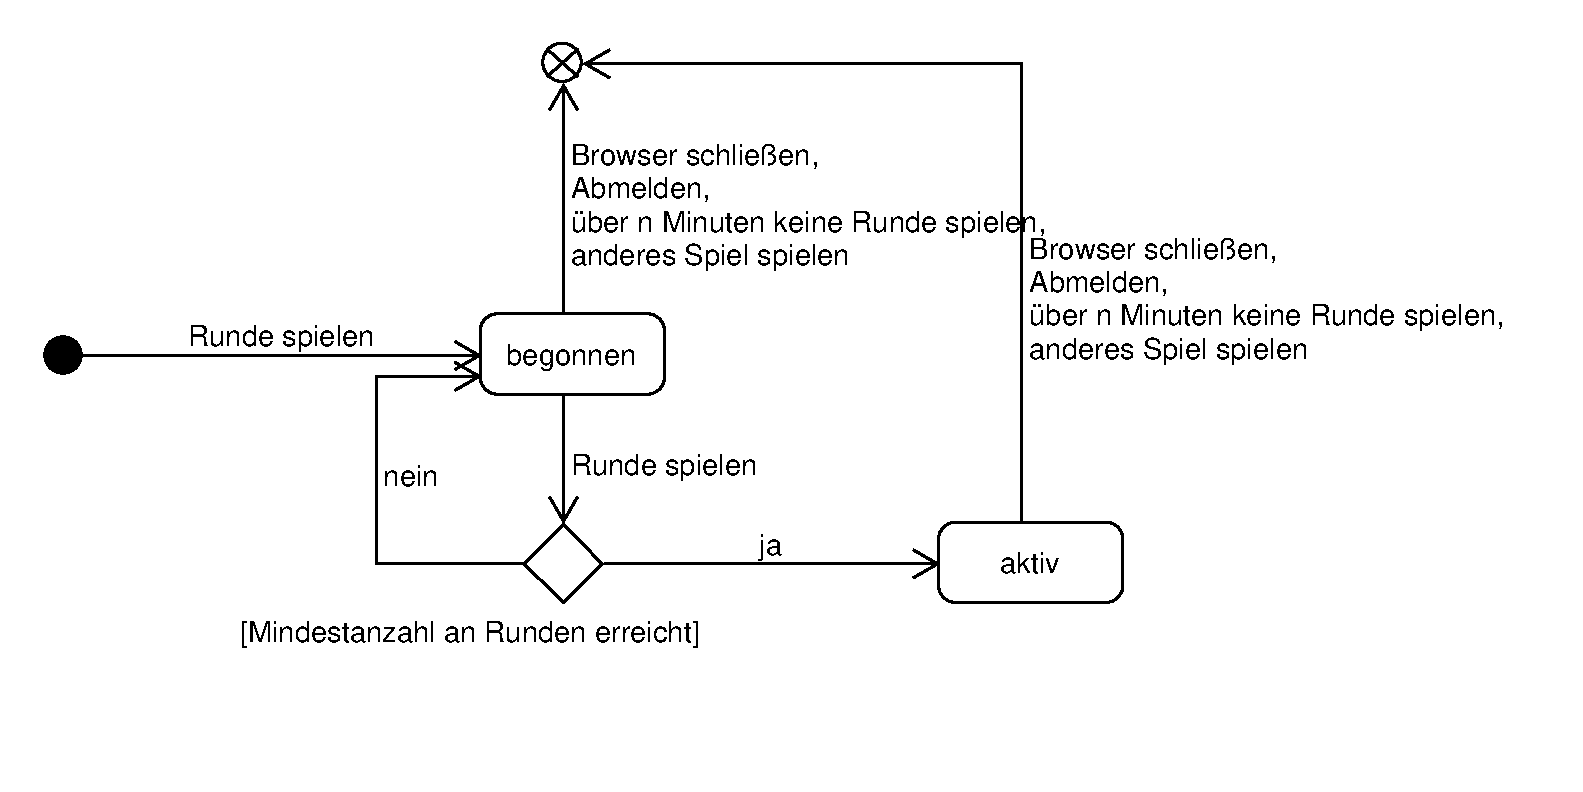
\includegraphics[width=\textwidth]{img/Streak_Zustand.pdf}
	Die Zustände, die eine Streak haben kann.
	Eine Streak ist immer auf einen Spieler beschränkt.
	Zustandsbeschreibung:
	\begin{itemize}
		\item begonnen: Eine angefangene Streak, die noch nicht lang genug ist um für den Spieler eine erhöhte Punktzahl zu erreichen.
		\item aktiv: Die Streak ist lang genug. In diesem Zustand erhält der Spieler doppelt so viele Punkte.
	\end{itemize}
	\section{Spiel}
	\label{fig:Spiel_State}
	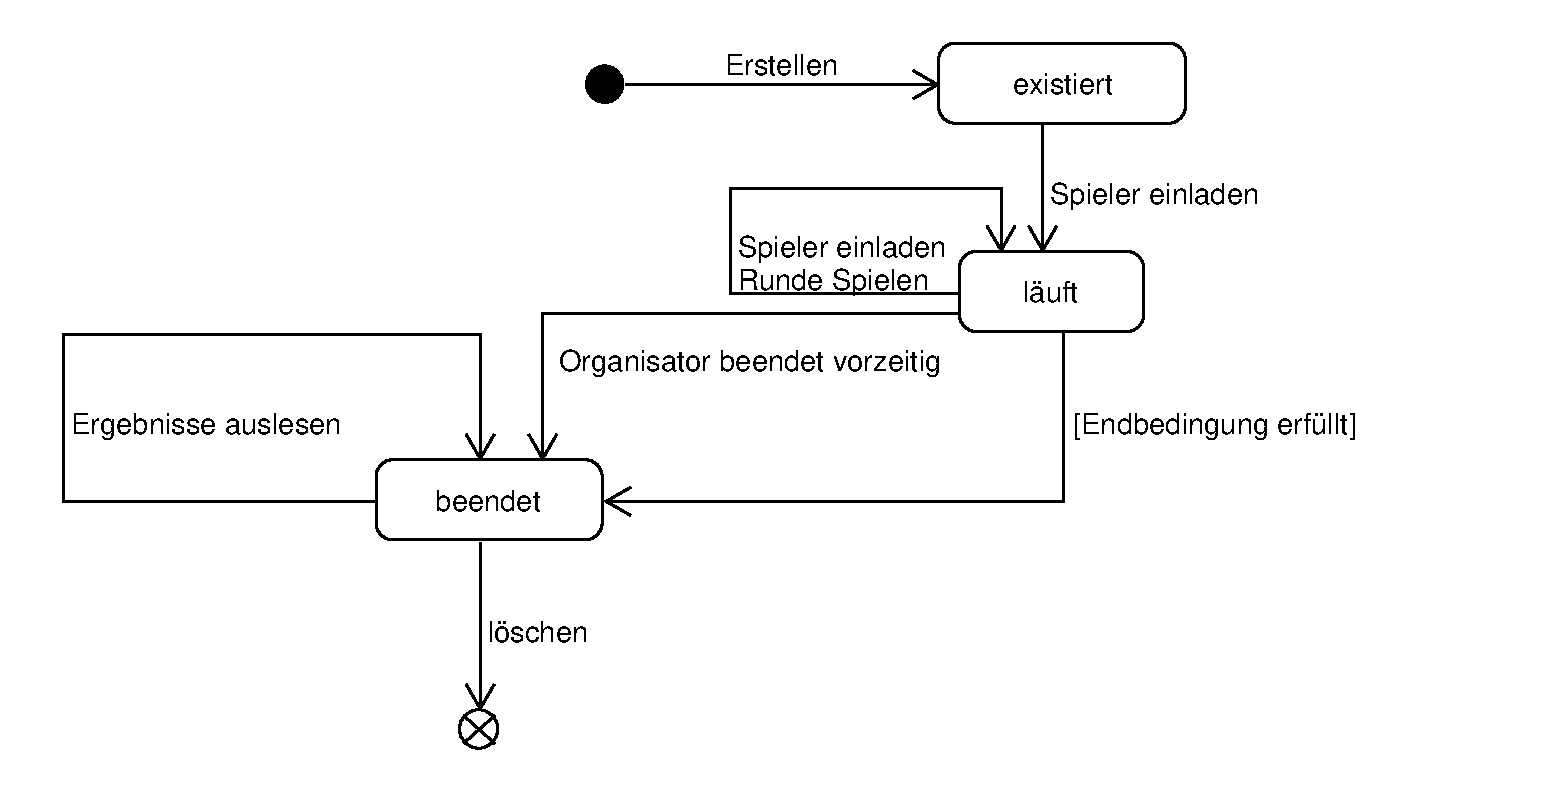
\includegraphics[width=\textwidth]{img/Spiel_Zustand.pdf}
	Die Zustände, die ein Spiel von der Erstellung bis zum Beenden haben kann.
	Zustandsbeschreibung:
	\begin{itemize}
		\item existiert: Das Spiel existiert, besitzt also einen Datensatz, Endbedingungen und Spielmodus. Es sind aber noch keine Spieler eingeladen, also kann es nicht gespielt werden.
		\item läuft: Das Spiel kann von Spielern gespielt werden.
		\item beendet: Das Spiel wurde beendet. Kein Spieler kann mehr spielen. Die Ergebnisse können jedoch noch ausgelesen werden.
	\end{itemize}
	\section{Achievements}
	\label{fig:Achievement_State}
	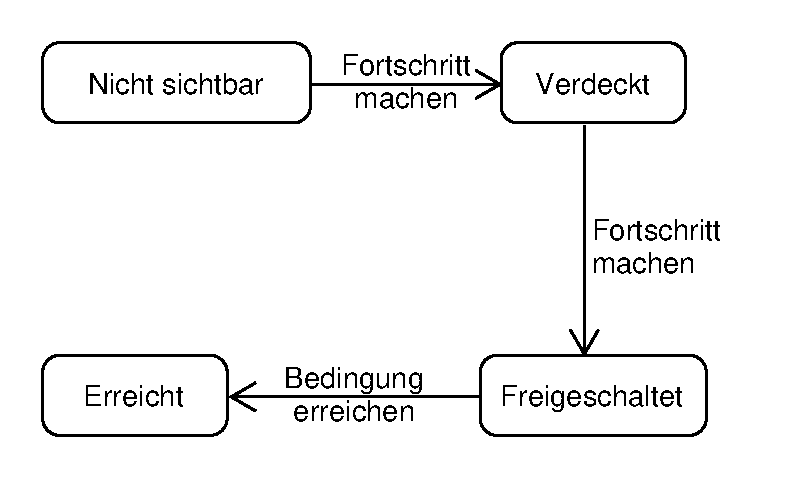
\includegraphics[width=\textwidth]{img/Achievement_State.pdf}
	Die Zustände, die ein Achievement von \enquote{Spieler kennt das Achievement nicht}, bis zu \enquote{Spieler hat das Achievement erreicht}, durchlaufen kann.
	\begin{itemize}
		\item Nicht sichtbar: Spieler weiß nicht, dass das Achievement existiert.
		\item Verdeckt: Spieler weiß dass dieses Achievement existiert, weiß jedoch nicht was er tun muss um es zu erreichen.
		\item Freigeschaltet: Die Bedingungen für das Erreichen dieses Achievements sind dem Spieler bekannt.
		\item Erreicht: Der Spieler hat die Bedingungen für das Erreichen dieses Achievements erfüllt.
	\end{itemize}

	\chapter{Gamification}
	Im Produkt wird eine Reihe von Gamification-Elementen umgesetzt.
	Eine Art dieser Elemente sind Achievements und Daily Challenges.
	Im Nachfolgenden werden die implementierten Achievements und Daily-Challenges aufgeführt.

	\section{Achievements}
	\hypertarget{Ach}{}

	\subsection{AchievementPlayRounds}
	Diese Achievements werden erreicht, wenn der Spiele eine bestimmte Anzahl an Runden gespielt hat. \\
	\begin{itemize}
		\item AchievementPlayOneRound
		\item AchievementPlayFiveRound
		\item AchievementPlayTenRound
		\item AchievementPlayFourtyTwoRound
		\item AchievementPlayHundredRound
	\end{itemize}

	\subsection{AchievementGetStreak}
	Diese Achievements werden erreicht, sobald der Spieler eine Streak in Höhe vom gegebenen Wert erreicht. \\
	\begin{itemize}
		\item AchievementGetStreakTwo
		\item AchievementGetStreakFive
		\item AchievementGetStreakTen
	\end{itemize}

	\newpage
	\subsection{AchievementCompleteDaily}
	Diese Achievements werden erreicht, wenn der Spieler eine bestimmte Anzahl an Daily-Challenges abschließt. \\
	\begin{itemize}
		\item AchievementCompleteOneDaily
		\item AchievementCompleteThreeDaily
		\item AchievementCompleteSevenDaily
	\end{itemize}

	\subsection{AchievementReachTotalScore}
	Diese Achievements werden erreicht, sobald die Gesamtpunktzahl einen bestimmten Wert erreicht. \\
	\begin{itemize}
		\item AchievementReachTotalScoreHundred
		\item AchievementReachTotalScoreTwoHundredFifty
		\item AchievementReachTotalScoreFiveHundred
		\item AchievementReachTotalScoreThousand
		\item AchievementReachTotalScoreTwoThousand
		\item AchievementReachTotalScoreFiveThousand
	\end{itemize}

	\subsection{AchievementReachRoundScore}
	Diese Achievements werden erreicht, wenn der Spieler eine bestimmte Anzahl an Punkten nach einer einzelnen Runde erreicht. Zusätzliche Punkte (z.B. durch) laufende Streaks werden hierbei nicht beachtet. \\
	\begin{itemize}
		\item AchievementReachRoundScoreSixty
		\item AchievementReachRoundScoreSeventy
		\item AchievementReachRoundScoreEighty
		\item AchievementReachRoundScoreNinety
	\end{itemize}


	\section{Daily-Challenges}
	\hypertarget{Daily}{}
	Die folgenden Daily-Challenges werden abgeschlossen, wenn der Spieler die Aufgabe an einem Tag erfüllt. \\
	\begin{itemize}
		\item DailyPlayThreeRounds
		\item DailyGetStreakThree
		\item DailyReachScoreHundredFifty
		\item DailyReachRoundScoreEighty
	\end{itemize}

	
	\chapter{Datenhaltung}

    \section{Ordnerstruktur}

    \subsection{WAR-Datei}
	In der WAR-Datei\footnote{Für eine genauere Beschreibung wird auf die \href{https://tomcat.apache.org/tomcat-7.0-doc/appdev/deployment.html\#Standard\_Directory\_Layout}{Tomcat-Dokumentation} verwiesen.}, die in den \$CATALINA\_HOME Ordner von Tomcat gelegt wird, müssen folgende Ordner und Dateien existieren:
    \begin{itemize}
        \item \texttt{*html, *jsp, etc.} \\Dies sind die statischen Dateien, die später direkt vom Browser aufrufbar sein müssen. Sie können auch in untergeordneten Ordnern liegen.
        \item \texttt{/WEB-INF/web.xml} \\Dies ist die Web Application Deployment Descriptor Datei für die Anwendung. In dieser werden die Routen für Anfragen an den Server festgelegt.
        \item \texttt{/WEB-INF/classes/} \\Hier liegen die Klassen des Produkts mit ihrer Paketstruktur.
        \item \texttt{/WEB-INF/lib/} \\Hier liegen alle 3rd-Party Bibliotheken.
    \end{itemize}
	\subsection{Stammverzeichnis}
	Weiterhin existiert ein Verzeichnis \texttt{/CSSELECT/}, in welchem das Produkt Daten sichert.
	Der Ort des Stammverzeichnisses wird in der Konfigurationsdatei angegeben.
	Im Verzeichnis \texttt{/CSSELECT/games/} erhält jedes Spiel einen Ordner seiner ID, in dem die Bilddateien der Graphen des Merkmalsdatensatzes gespeichert werden.
	
	\section{Konfiguration}
	Die Konfigurationsdatei enthält alle Einstellungsmöglichkeiten, die das Produkt betreffen in Form von Key-Value-Paaren:
	Die Konfigurationsdatei muss zu Anwendungsstart im Verzeichnis \texttt{/} liegen. % TODO Pfad eintragen
	\begin{itemize}
		\item organiserpassword \\Das Passwort, das ein Organisator bei der Registrierung angeben muss.
		\item mlserverurl       \\Die URL, unter der der ML-Server zu erreichen ist.
		\item homedirectory     \\Das Verzeichnis, unter dem Daten auf der Festplatte abgelegt werden sollen.
		\item database          \\Kategorie für die Datenbankeinstellungen.
		\begin{itemize}
			\item type          \\Typ der zu verwendenden Datenbank, Standard ist MySQL.
			\item hostname      \\Hostname unter dem der Datenbankserver erreichbar ist.
			\item port          \\Port des Datenbankservers.
			\item username      \\Nutzername des Datenbankbenutzers.
			\item password      \\Passwort des Datenbankbenutzers.
		\end{itemize}
	\end{itemize}

	\section{Datenbank}
	In der Datenbank werden sämtliche spielrelevanten Daten gesichert.
	Die Standardimplementierung verwendet eine MySQL-Datenbank mit folgender geplanter Strukturierung der Daten:
	Das Produkt verwendet eine Datenbank für seine Daten (fortan Hauptdatenbank genannt) sowie für jedes Spiel eine vom Organisator angegebene Datenbank.
	\subsection{Spielerdaten}
	Eine Tabelle in der Hauptdatenbank hält die Daten für die Spieler.
	Die einzelnen Spalten sind dabei die Folgenden:
	\begin{itemize}
		\item ID
		\item Username
		\item E-Mail-Addresse
		\item Passwort-Hash
		\item Passwort-Salt
		\item Score (Gesamt erreichte Punkte des Spielers)
		\item Anzahl gespielter Spiele
	\end{itemize}
	\subsection{Organisatordaten}
	Eine weitere Tabelle in der Hauptdatenbank hält die Daten der Organisatoren.
	Die einzelnen Spalten sind dabei die Folgenden:
	\begin{itemize}
		\item ID
		\item Username
		\item E-Mail-Addresse
		\item Passwort-Hash
		\item Passwort-Salt
	\end{itemize}
	Weiterhin gibt es eine weitere Tabelle mit den gesicherten Spieleinstellungen.
	\begin{itemize}
		\item Titel der Voreinstellung
		\item Organisator-ID, dem die Voreinstellung gehört
		\item Beschreibung
		\item Art der Spielterminierung
		\item Spielmodus
		\item Name der zu nutzenden Datenbank
		\item Eingeladene Spieler
	\end{itemize}
	\subsection{Merkmalsdatensätze}
	Jeder Merkmalsdatensatz erhält eine eigene Tabelle mit folgenden Inhalten:
	\begin{itemize}
		\item ID
		\item Dataset-Feature (Interner Name des Features)
		\item Englischer Name
		\item Englische Beschreibung
		\item Deutscher Name
		\item Deutsche Beschreibung
		\item Anteil fehlender Werte
		\item Beispielwerte
		\item Sechs Statistiken für numerische Merkmale
	\end{itemize}
	Die zum Merkmalsdatensatz zugehörigen Graphen werden auf der Festplatte in einem Verzeichnis gespeichert.
	\subsection{Spieldaten}
	Die grundlegenden Daten zum Spiel werden in einer Tabelle in der Hauptdatenbank verwaltet.
	\begin{itemize}
		\item ID
        \item ID des zugehörigen Organisators
		\item Titel
		\item Beschreibung
		\item Datenbankname
		\item Terminierungsstatus
		\item Spielmodus
	\end{itemize}
	Jedem Spiel wird vom Organisator eine eigene Datenbank zugewiesen.
	Löscht ein Organisator ein Spiel, so wird lediglich dessen Eintrag in voriger Tabelle gelöscht.
	Die spieleigene Datenbank bleibt hierbei unverändert.
	Die spieleigene Datenbank sichert die restlichen Daten der Game-Klasse, die nicht von obiger Tabelle erfasst werden.


	\chapter{Anhang}
	\section{Komplettes Klassendiagramm}
	%TODO: Komplettes Klassendiagramm als .svg (steht in Tipps)

\end{document}
